\chapter{Appendix} 
\label{cha:appendix}

In this chapter all remaining plots regarding the hyper-parameter optimizations are depicted for the sake of completeness.

\section{Swarm Velocities}
\label{app:velocity}
Velocity plots encompass fig. \ref{fig:stator_vel},  \ref{fig:pm_vel},  \ref{fig:yoke_vel},  \ref{fig:teeth_vel} and  \ref{fig:winding_vel}.
\begin{figure}[!hbt]
	\centering
	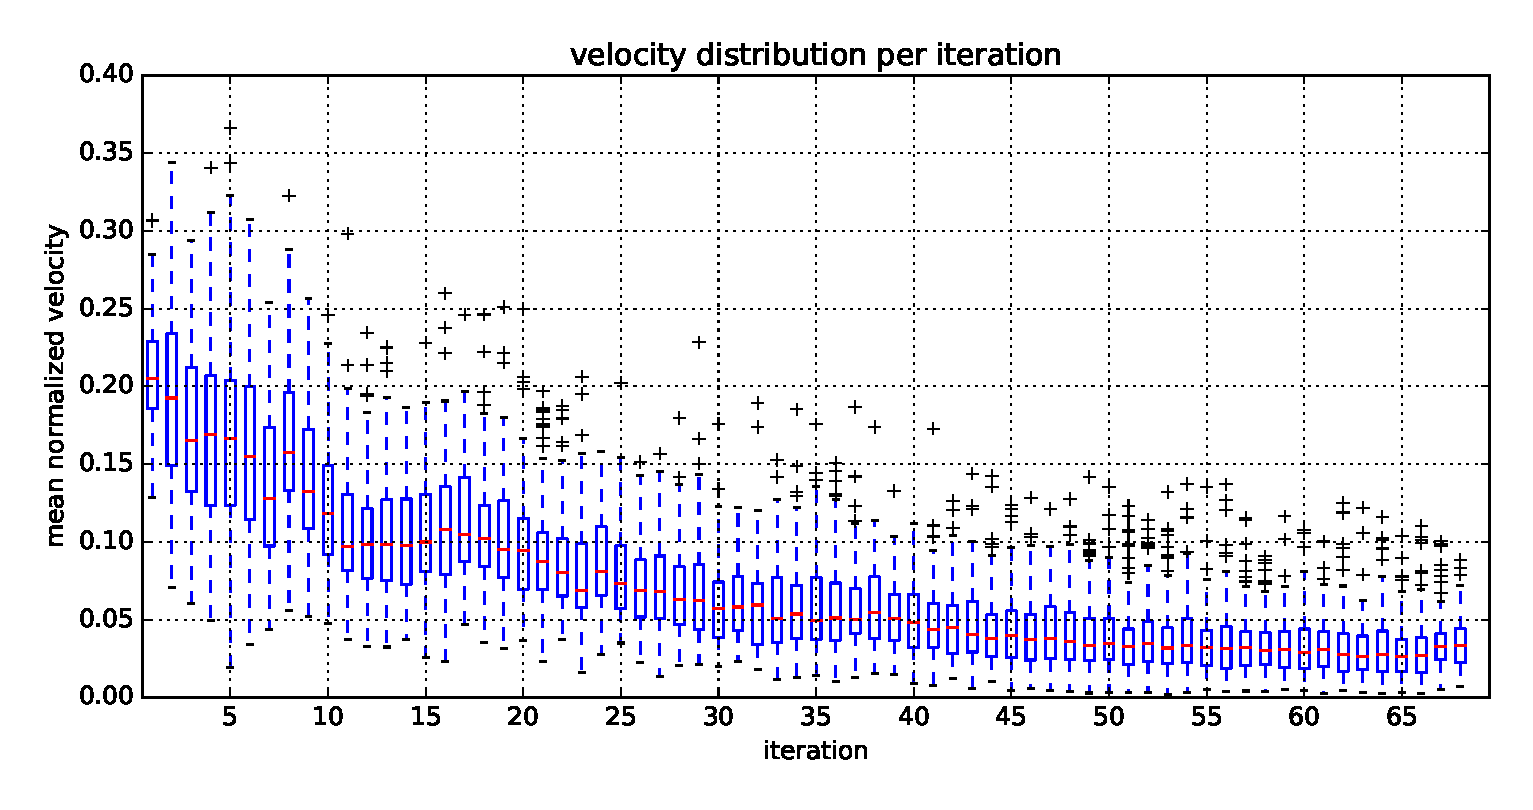
\includegraphics[width=\columnwidth]{evaluation/stator_vel.eps}
	\caption{Mean absolute velocity of the swarm's particles (from experiment 2)}
	\label{fig:stator_vel}
\end{figure}
\begin{figure}[!hbt]
	\centering
	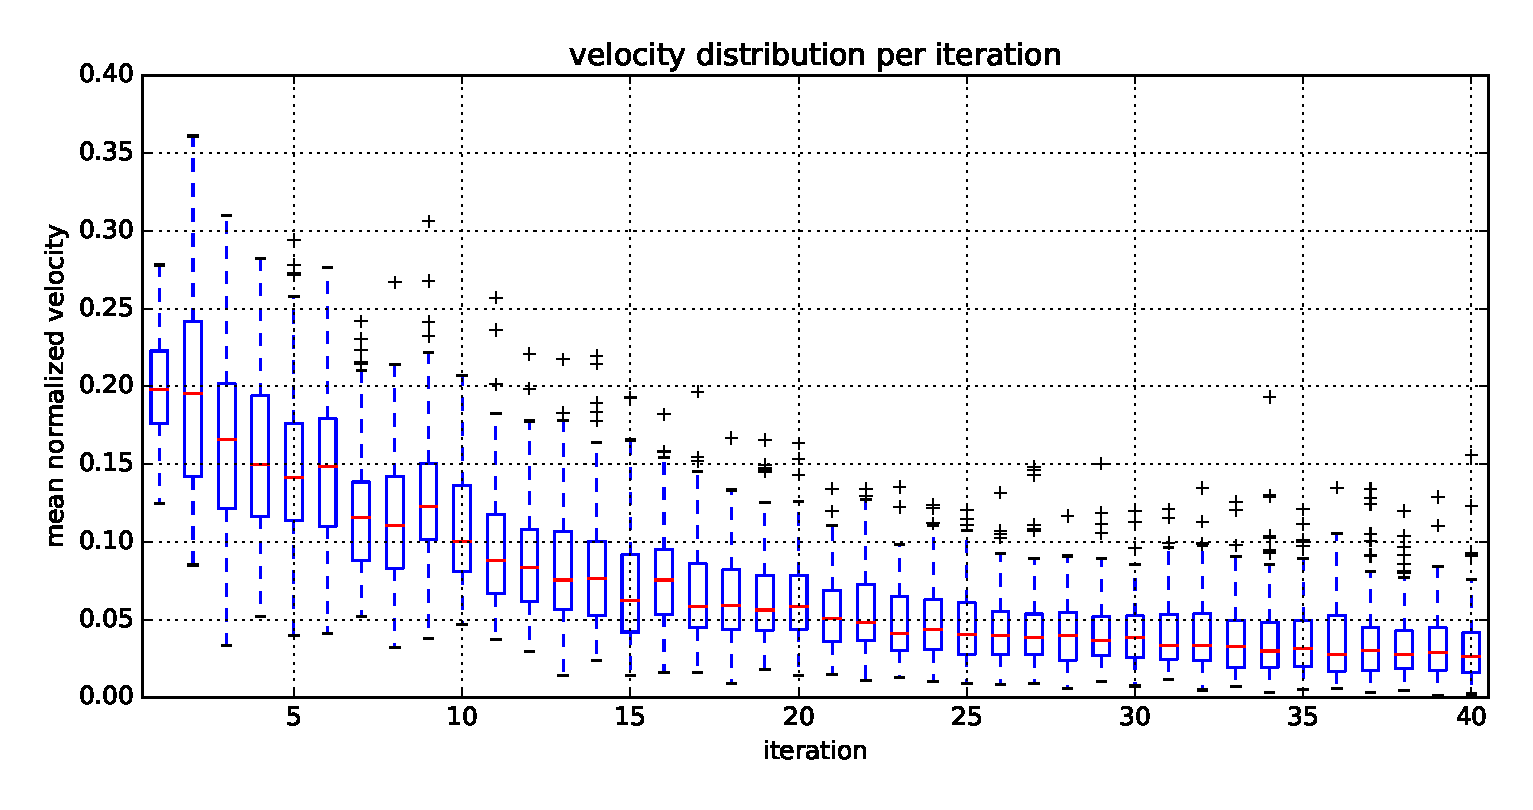
\includegraphics[width=\columnwidth]{evaluation/pm_vel.eps}
	\caption{Mean absolute velocity of the swarm's particles (from experiment 3)}
	\label{fig:pm_vel}
\end{figure}
\begin{figure}[!hbt]
	\centering
	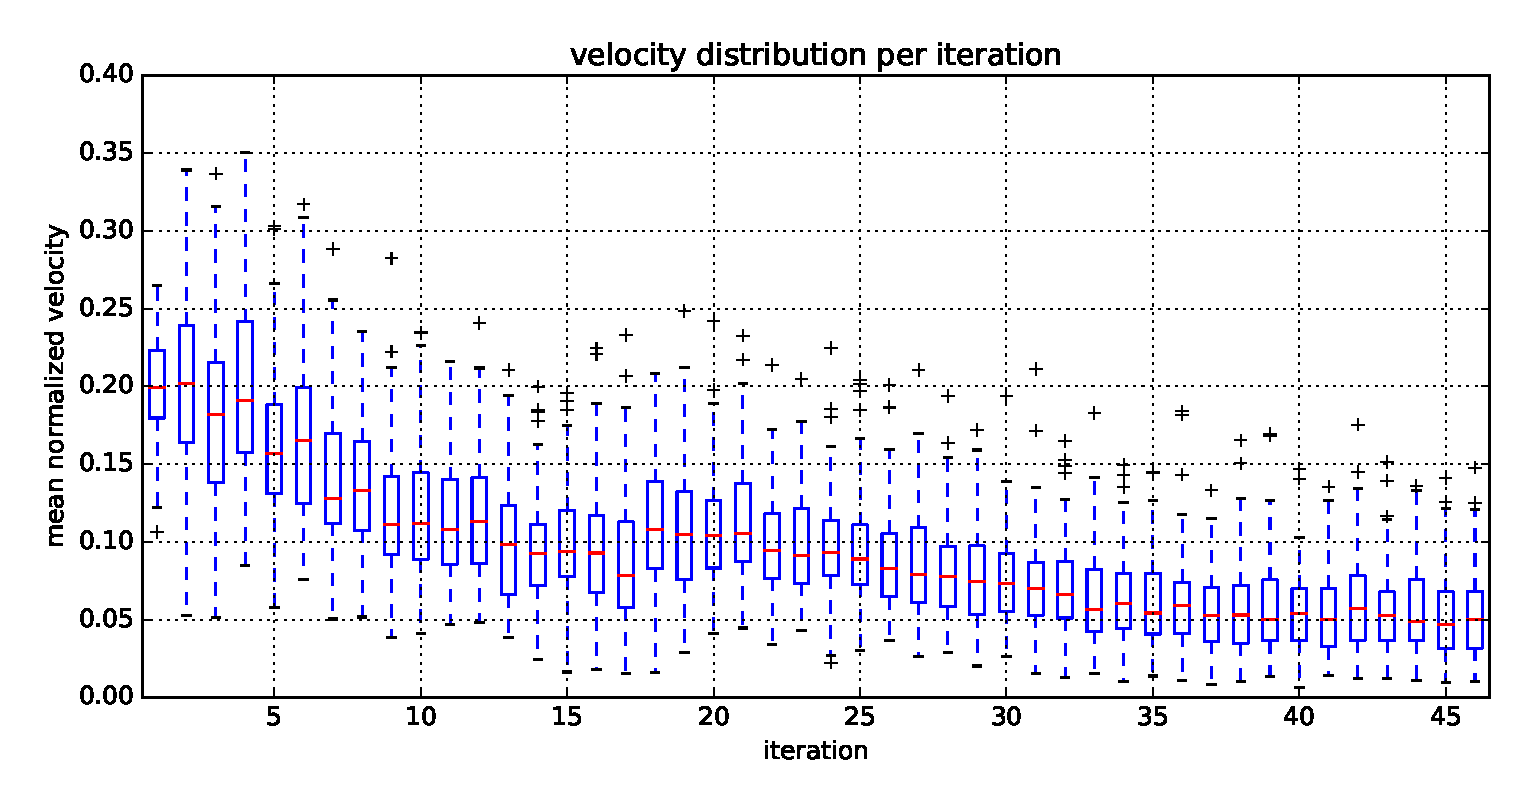
\includegraphics[width=\columnwidth]{evaluation/yoke_vel.eps}
	\caption{Mean absolute velocity of the swarm's particles (from experiment 4)}
	\label{fig:yoke_vel}
\end{figure}
\begin{figure}[!hbt]
	\centering
	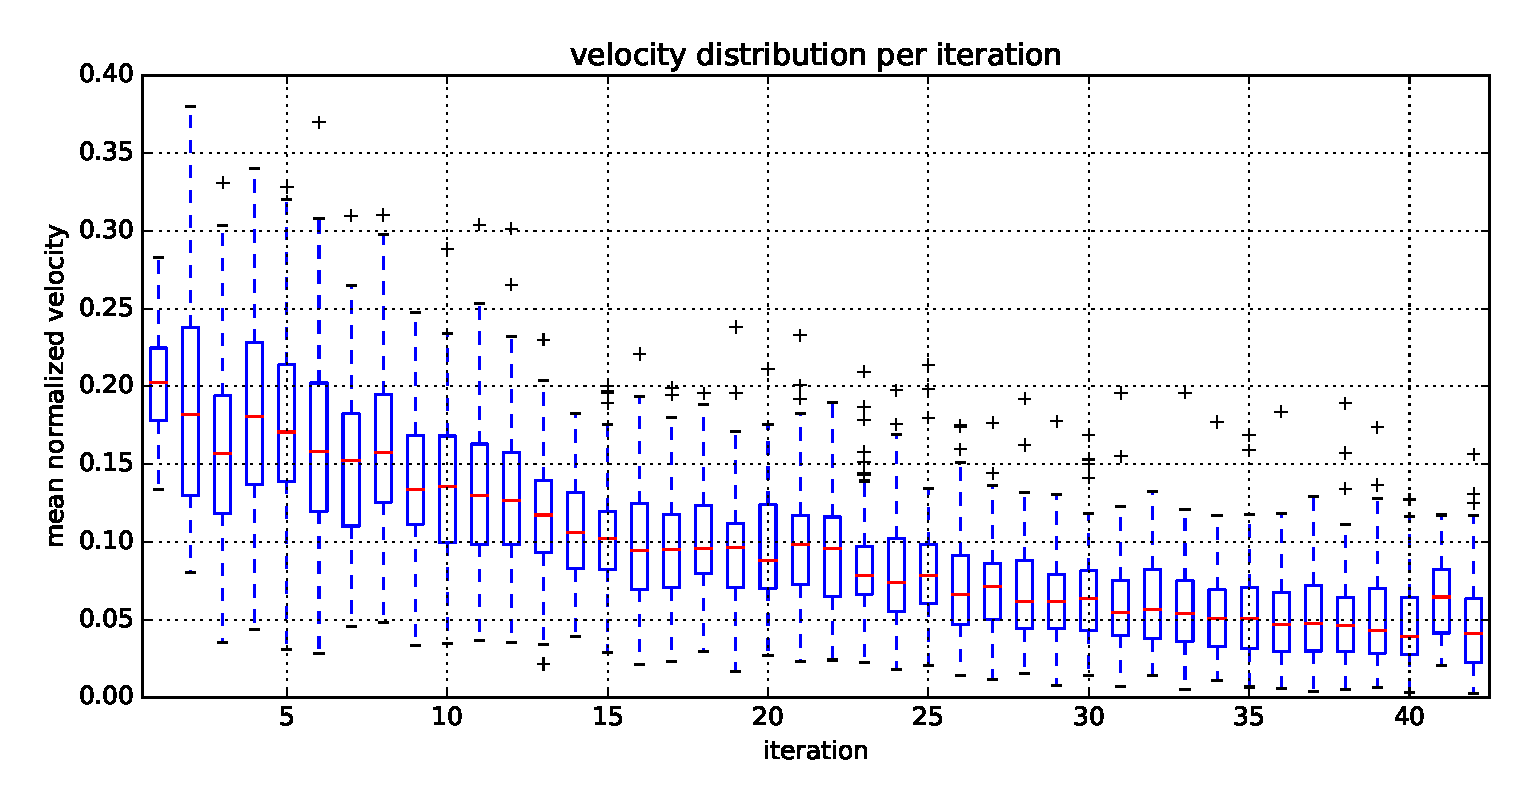
\includegraphics[width=\columnwidth]{evaluation/teeth_vel.eps}
	\caption{Mean absolute velocity of the swarm's particles (from experiment 5)}
	\label{fig:teeth_vel}
\end{figure}
\begin{figure}[!hbt]
	\centering
	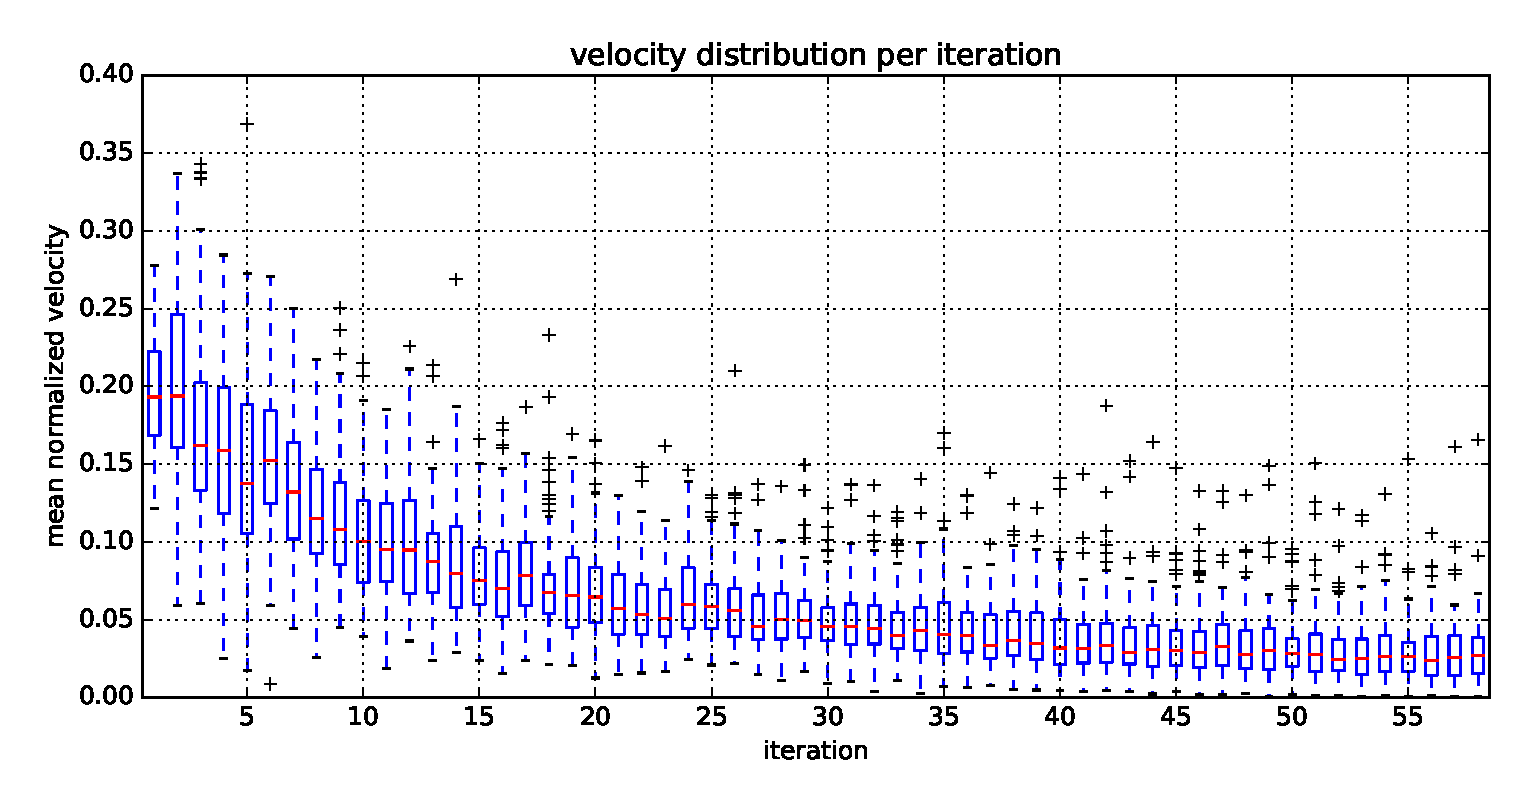
\includegraphics[width=\columnwidth]{evaluation/winding_vel.eps}
	\caption{Mean absolute velocity of the swarm's particles (from experiment 6)}
	\label{fig:winding_vel}
\end{figure}\clearpage

\section{Swarm Evaluation Trends}
\label{app:evaluation}
Evaluation plots encompass fig. \ref{fig:stator_eval}, \ref{fig:pm_eval}, \ref{fig:yoke_eval}, \ref{fig:teeth_eval} and \ref{fig:winding_eval}.
\begin{figure}[!hbt]
	\centering
	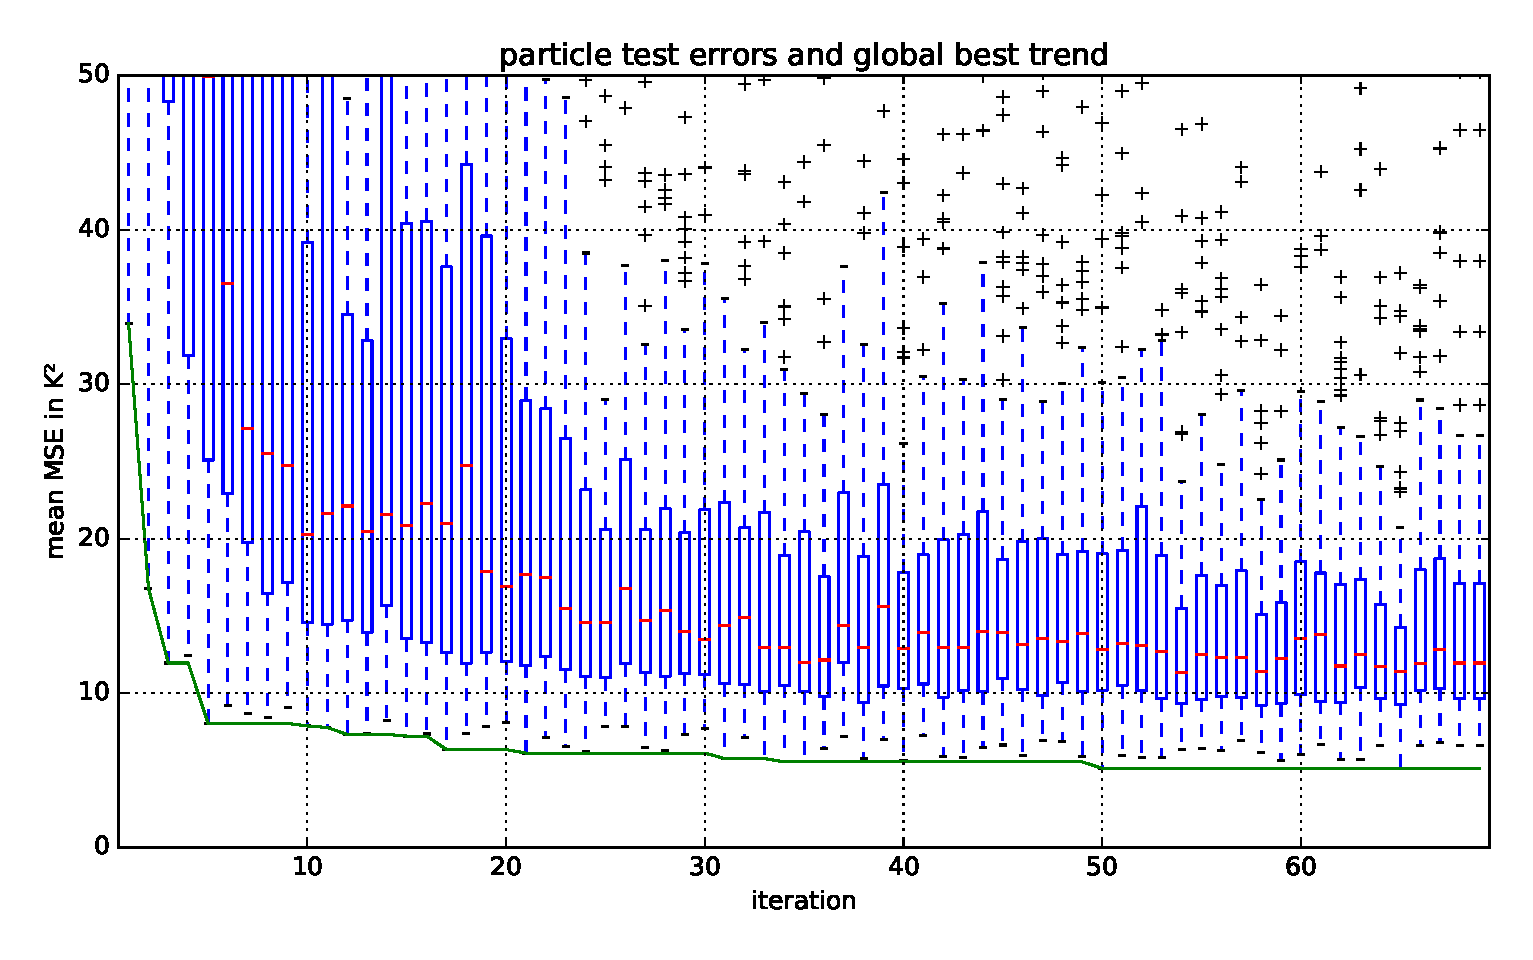
\includegraphics[width=\columnwidth]{evaluation/stator_eval.eps}
	\caption{Particle test scores over all iterations as box plots and the found best site's score as green line (from experiment 2)}
	\label{fig:stator_eval}
\end{figure}
\begin{figure}[!hbt]
	\centering
	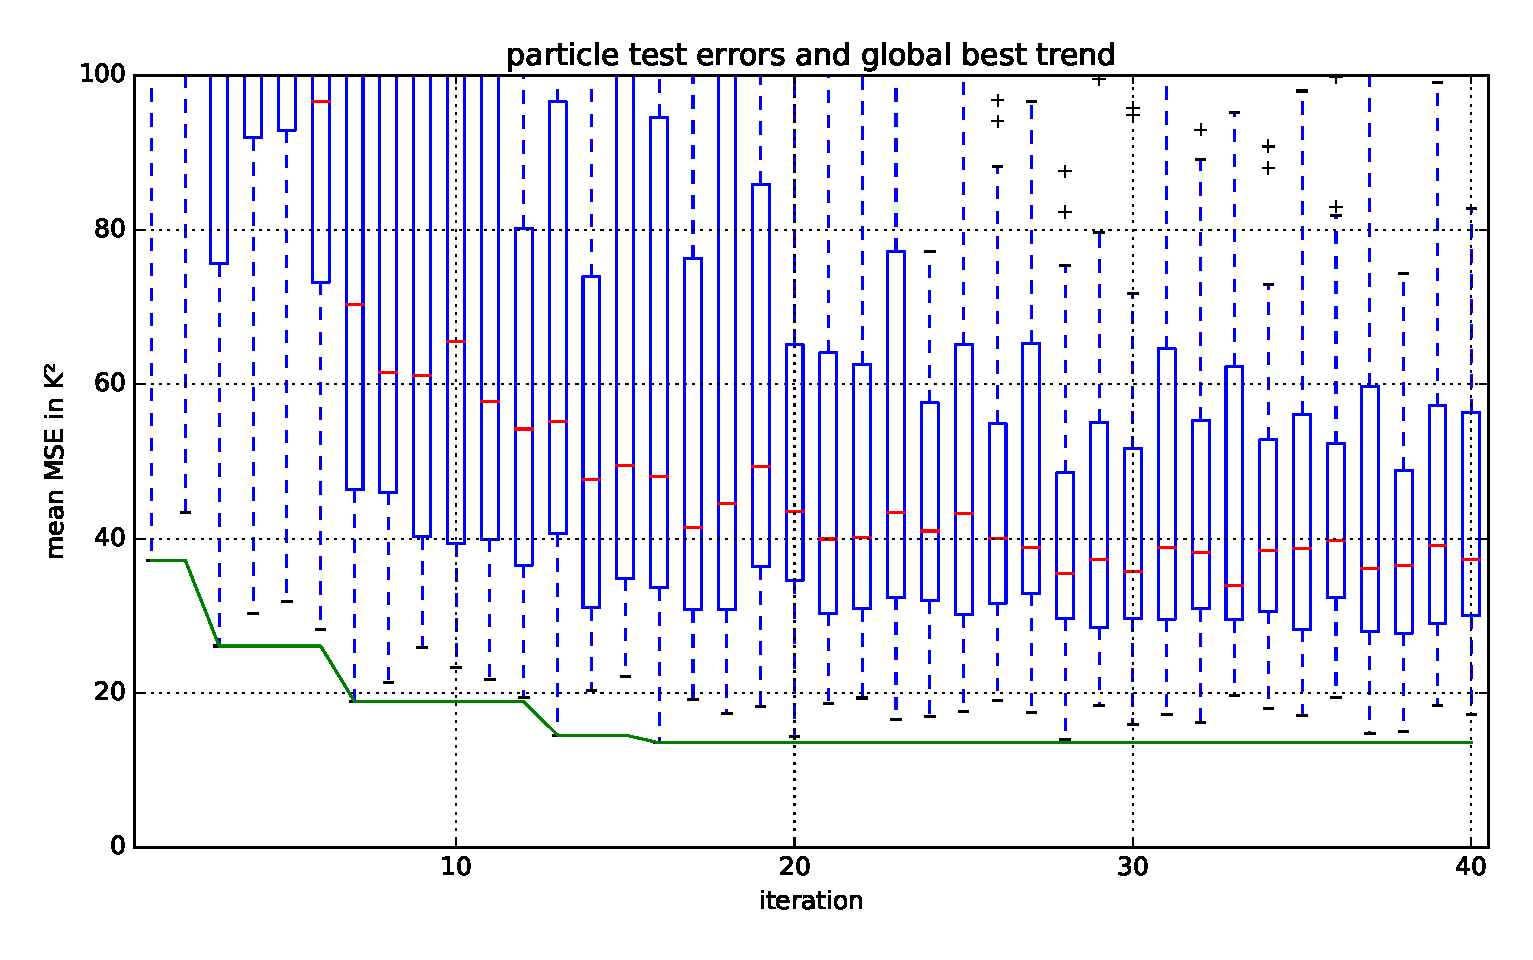
\includegraphics[width=\columnwidth]{evaluation/pm_eval.eps}
	\caption{Particle test scores over all iterations as box plots and the found best site's score as green line (from experiment 3)}
	\label{fig:pm_eval}
\end{figure}
\begin{figure}[!hbt]
	\centering
	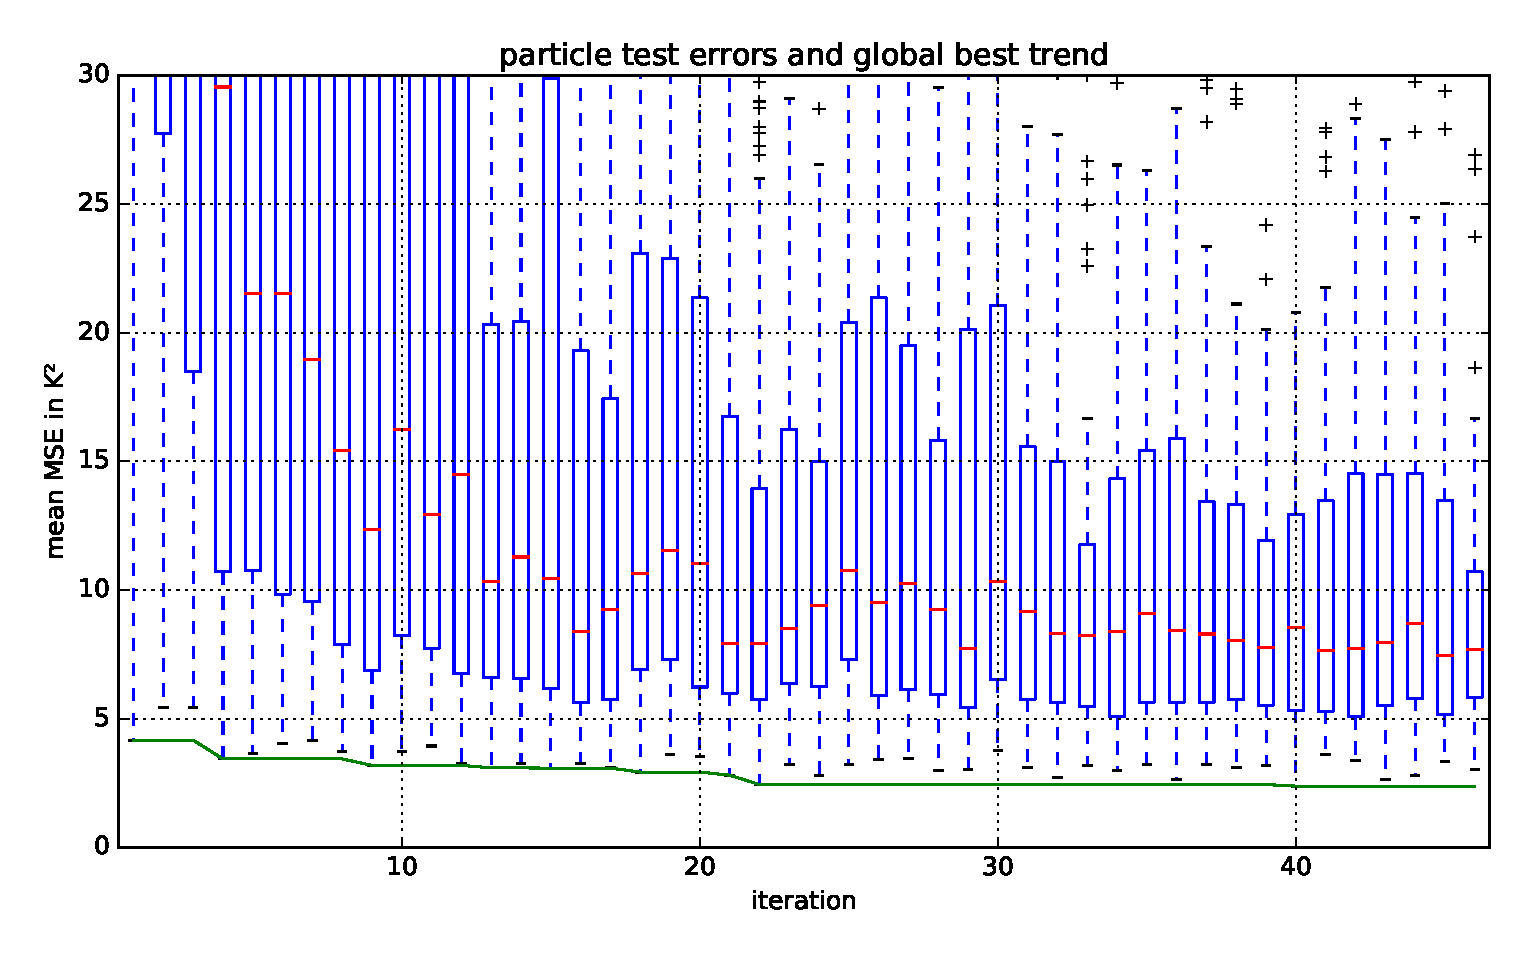
\includegraphics[width=\columnwidth]{evaluation/yoke_eval.eps}
	\caption{Particle test scores over all iterations as box plots and the found best site's score as green line (from experiment 4)}
	\label{fig:yoke_eval}
\end{figure}
\begin{figure}[!hbt]
	\centering
	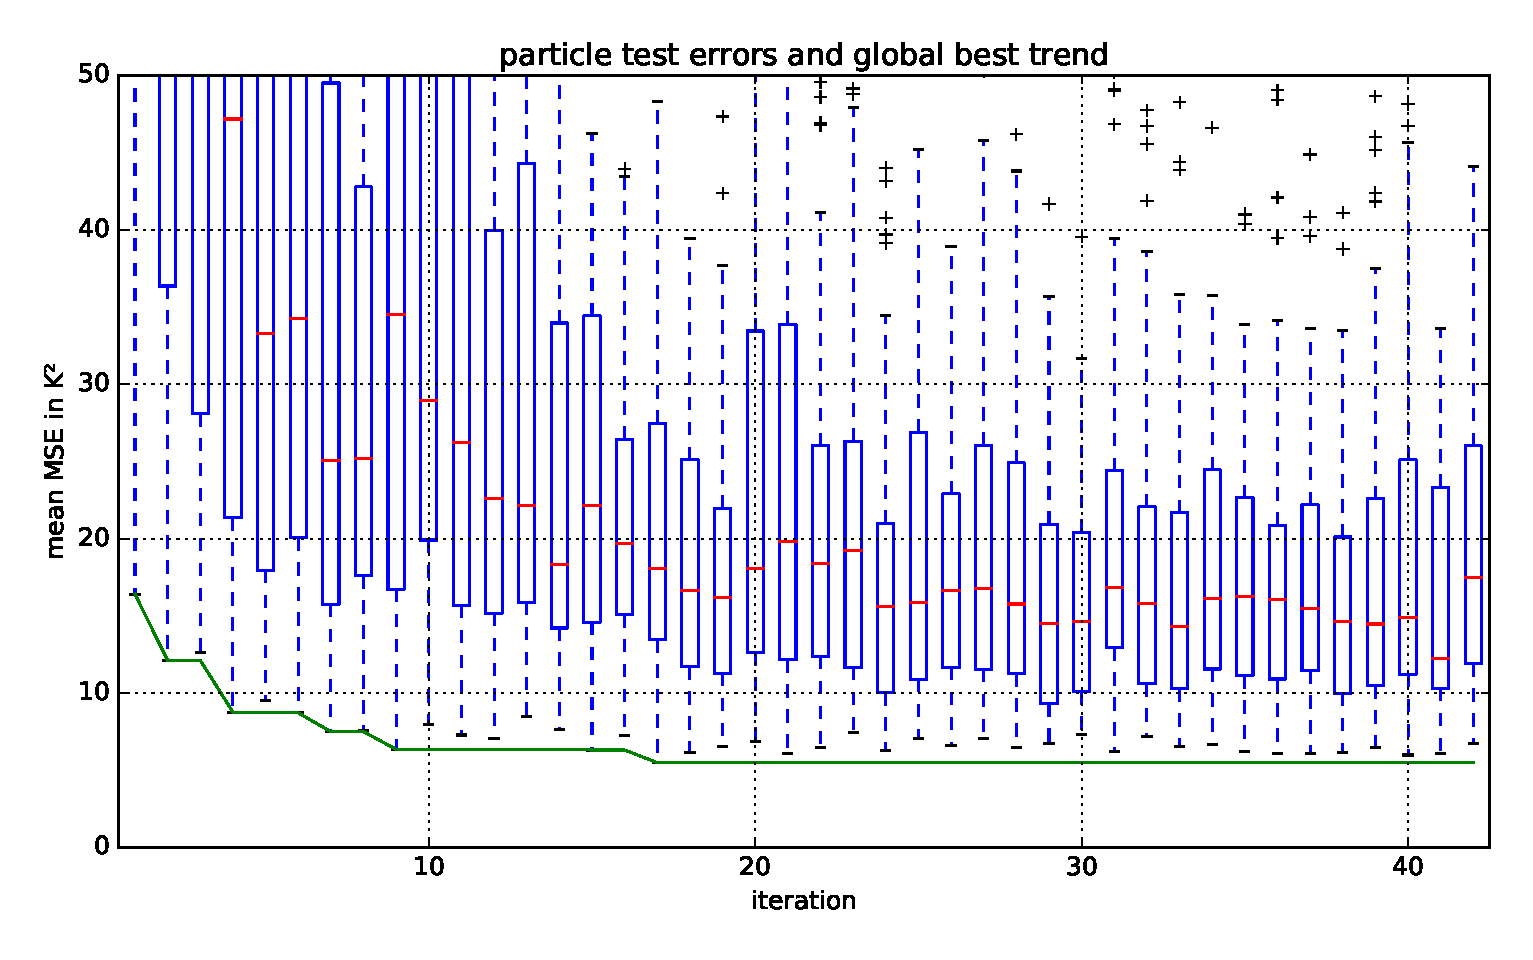
\includegraphics[width=\columnwidth]{evaluation/teeth_eval.eps}
	\caption{Particle test scores over all iterations as box plots and the found best site's score as green line (from experiment 5)}
	\label{fig:teeth_eval}
\end{figure}
\begin{figure}[!hbt]
	\centering
	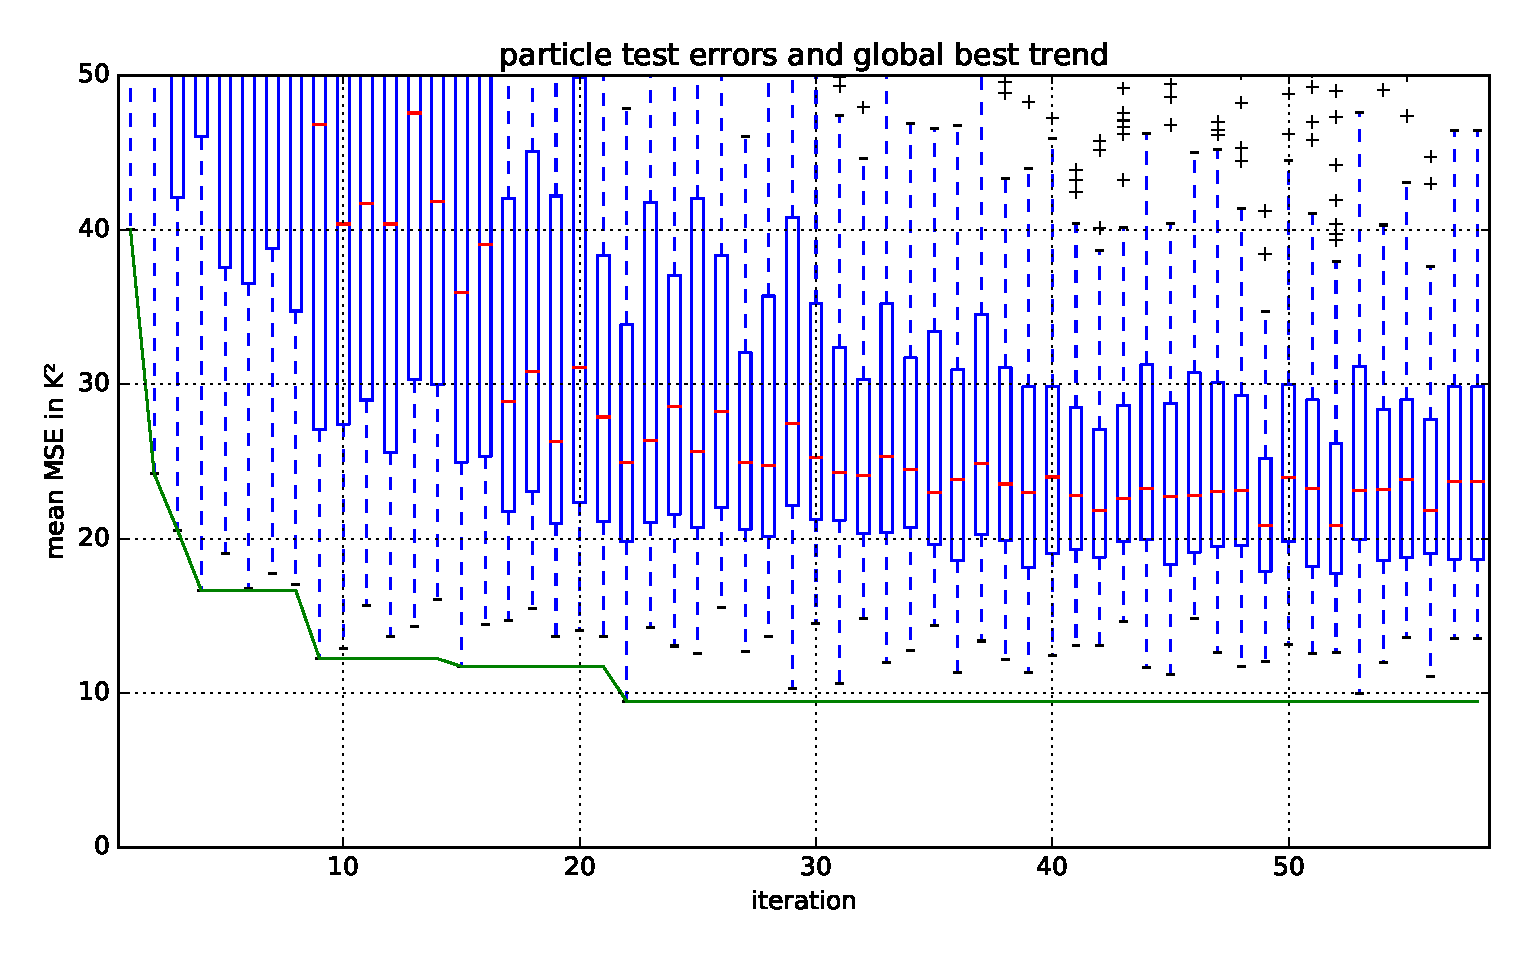
\includegraphics[width=\columnwidth]{evaluation/winding_eval.eps}
	\caption{Particle test scores over all iterations as box plots and the found best site's score as green line (from experiment 6)}
	\label{fig:winding_eval}
\end{figure}\clearpage

\section{Parameter Distributions}
\label{app:param_dist}
Distribution plots encompass fig. \ref{fig:stator_param_dist}, \ref{fig:pm_param_dist}, \ref{fig:yoke_param_dist}, \ref{fig:teeth_param_dist} and \ref{fig:winding_param_dist}.
\begin{figure}[!hbt]
	\centering
	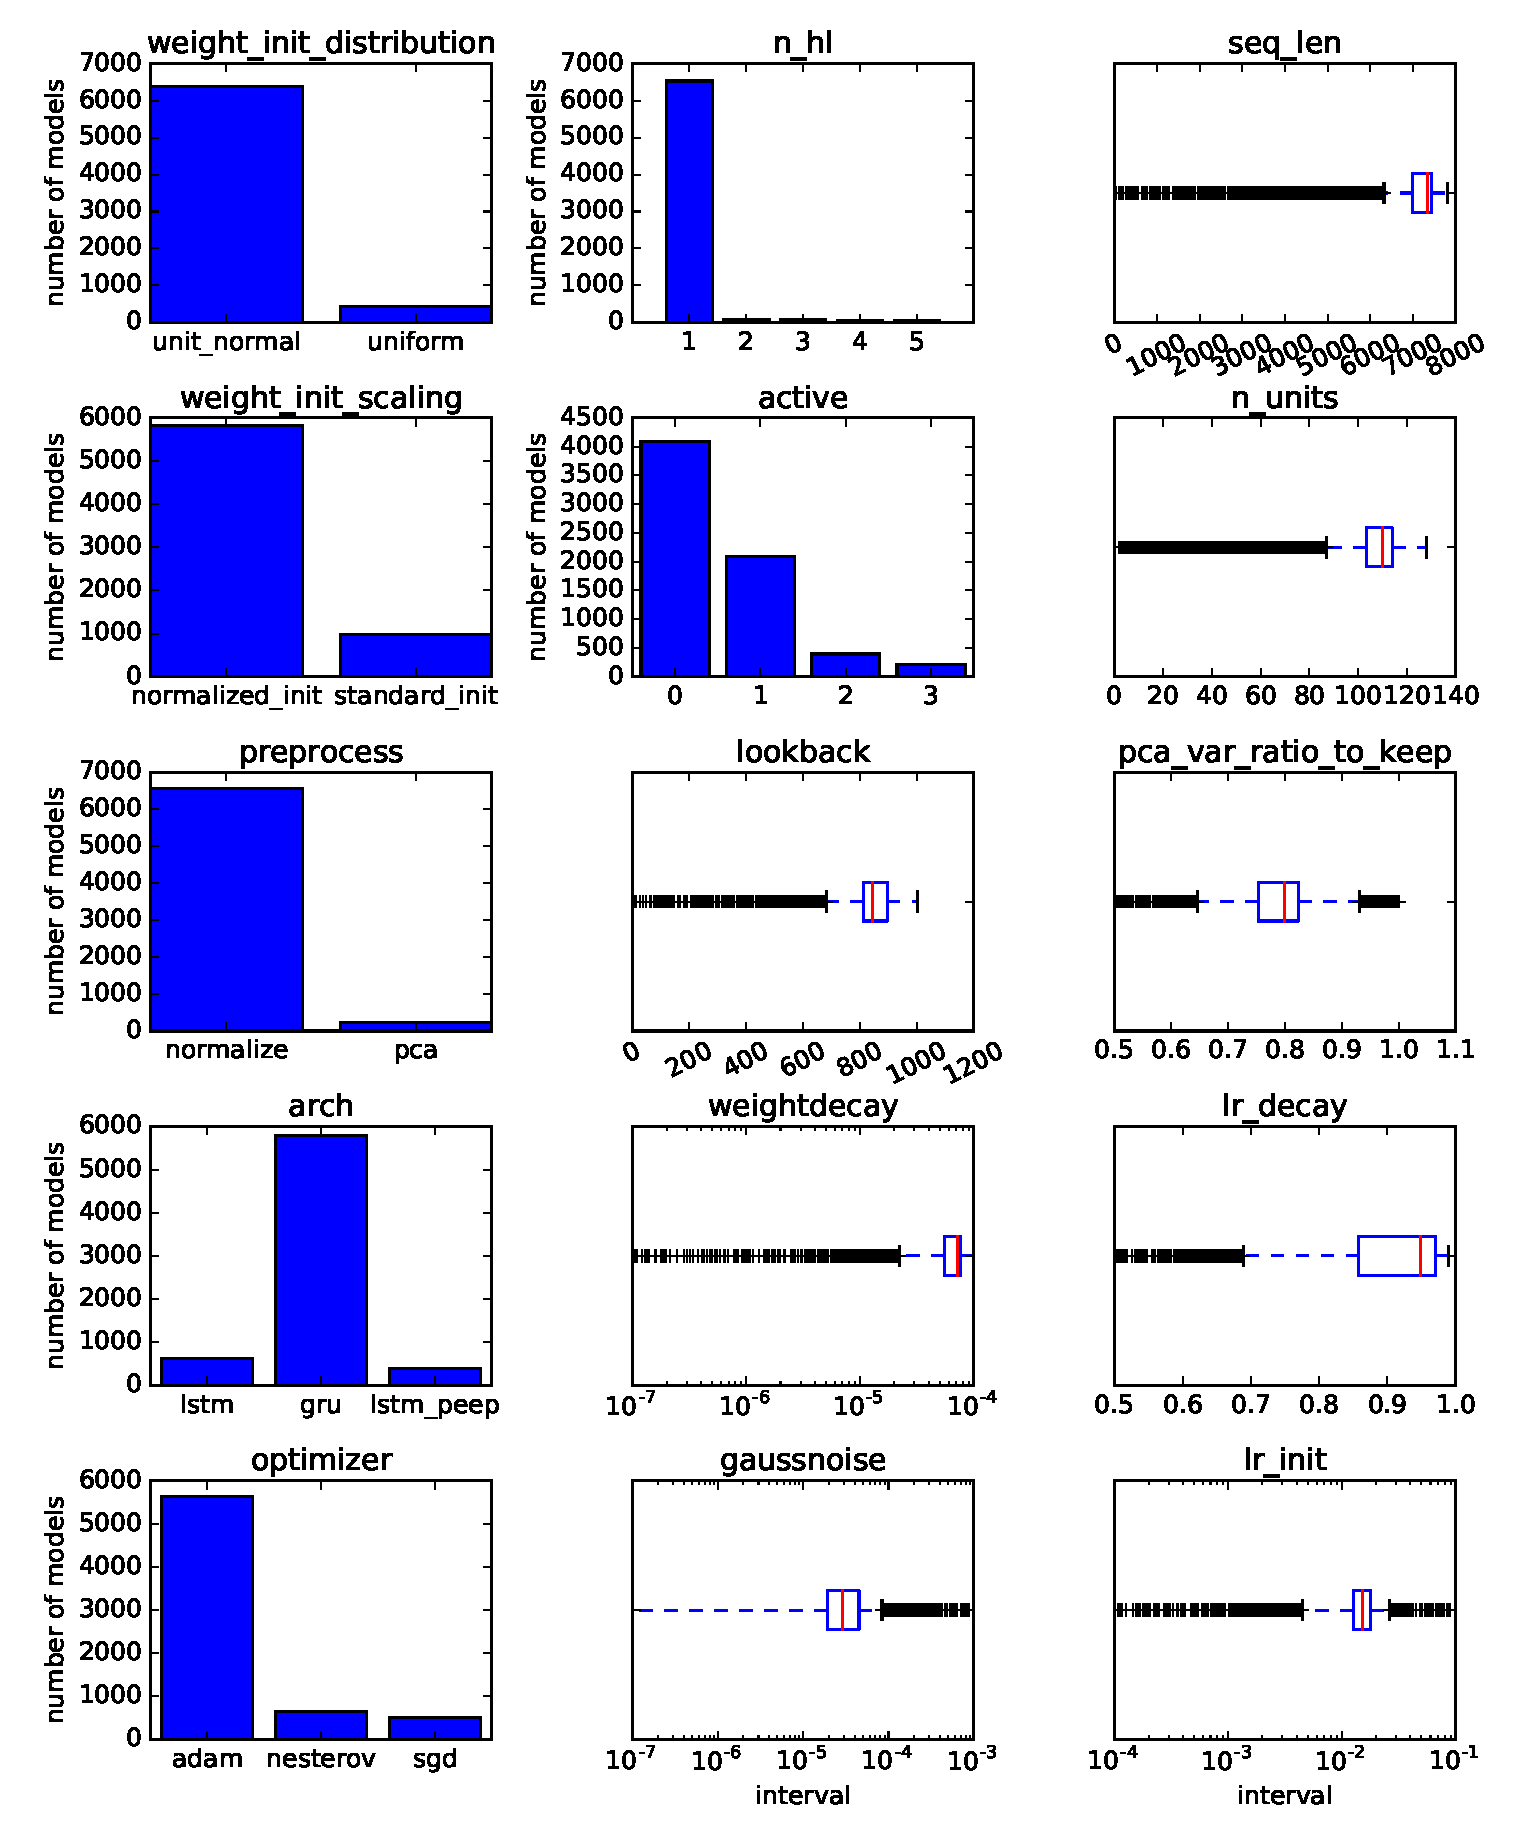
\includegraphics[width=\columnwidth]{evaluation/stator_paramdist.eps}
	\caption{Bar plots and box plots depicting the distribution of each hyper-parameter over all \gls{pso} iterations (from experiment 2)}
	\label{fig:stator_param_dist}
\end{figure}
\begin{figure}[!hbt]
	\centering
	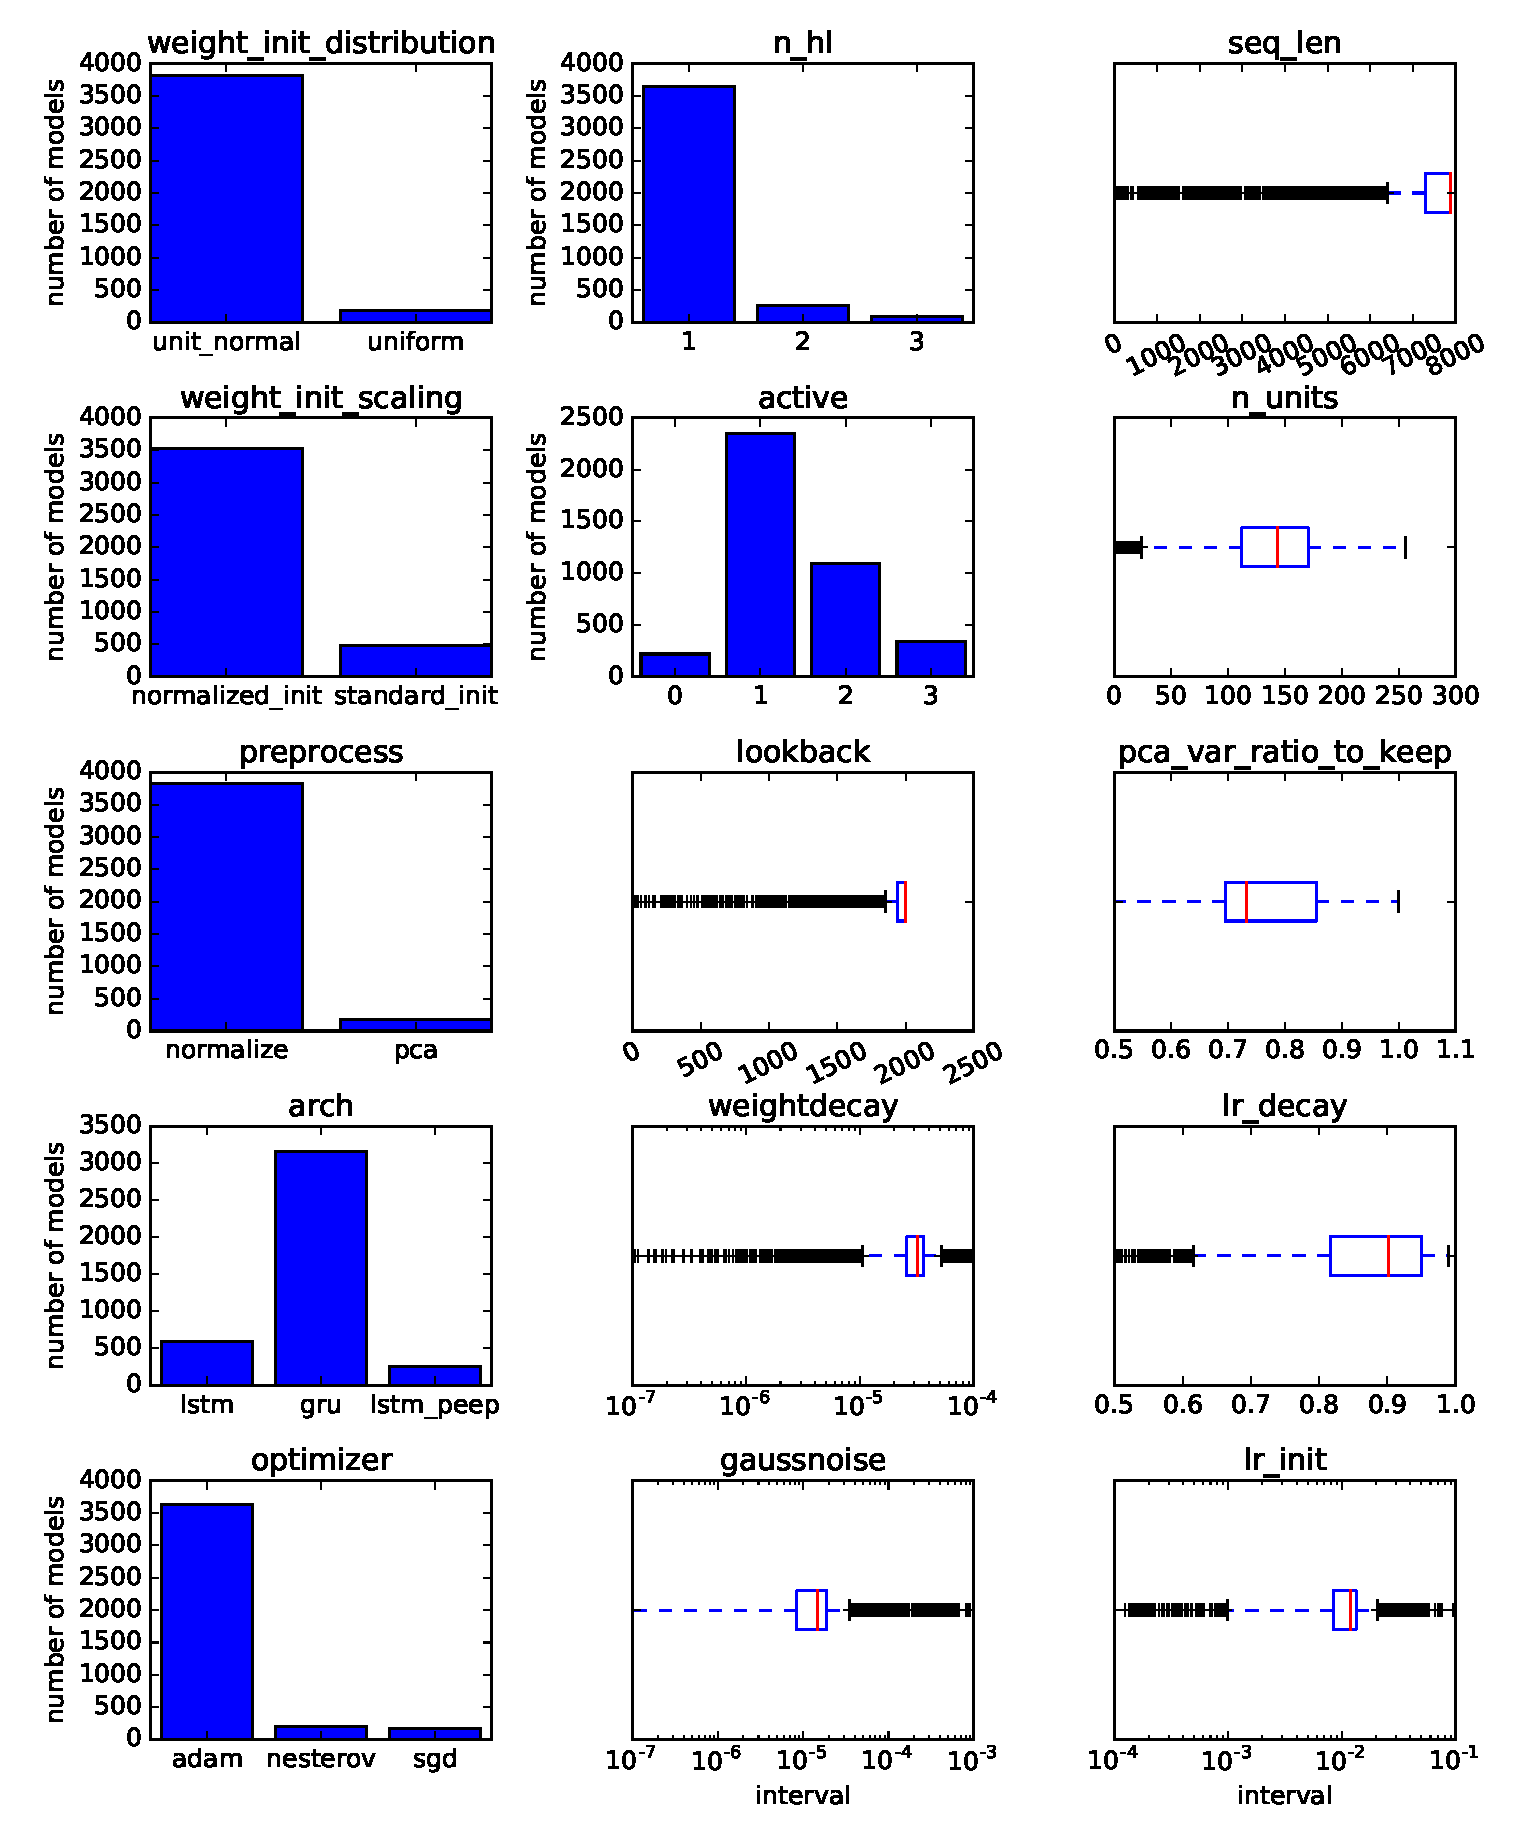
\includegraphics[width=\columnwidth]{evaluation/pm_paramdist.eps}
	\caption{Bar plots and box plots depicting the distribution of each hyper-parameter over all \gls{pso} iterations (from experiment 3)}
	\label{fig:pm_param_dist}
\end{figure}
\begin{figure}[!hbt]
	\centering
	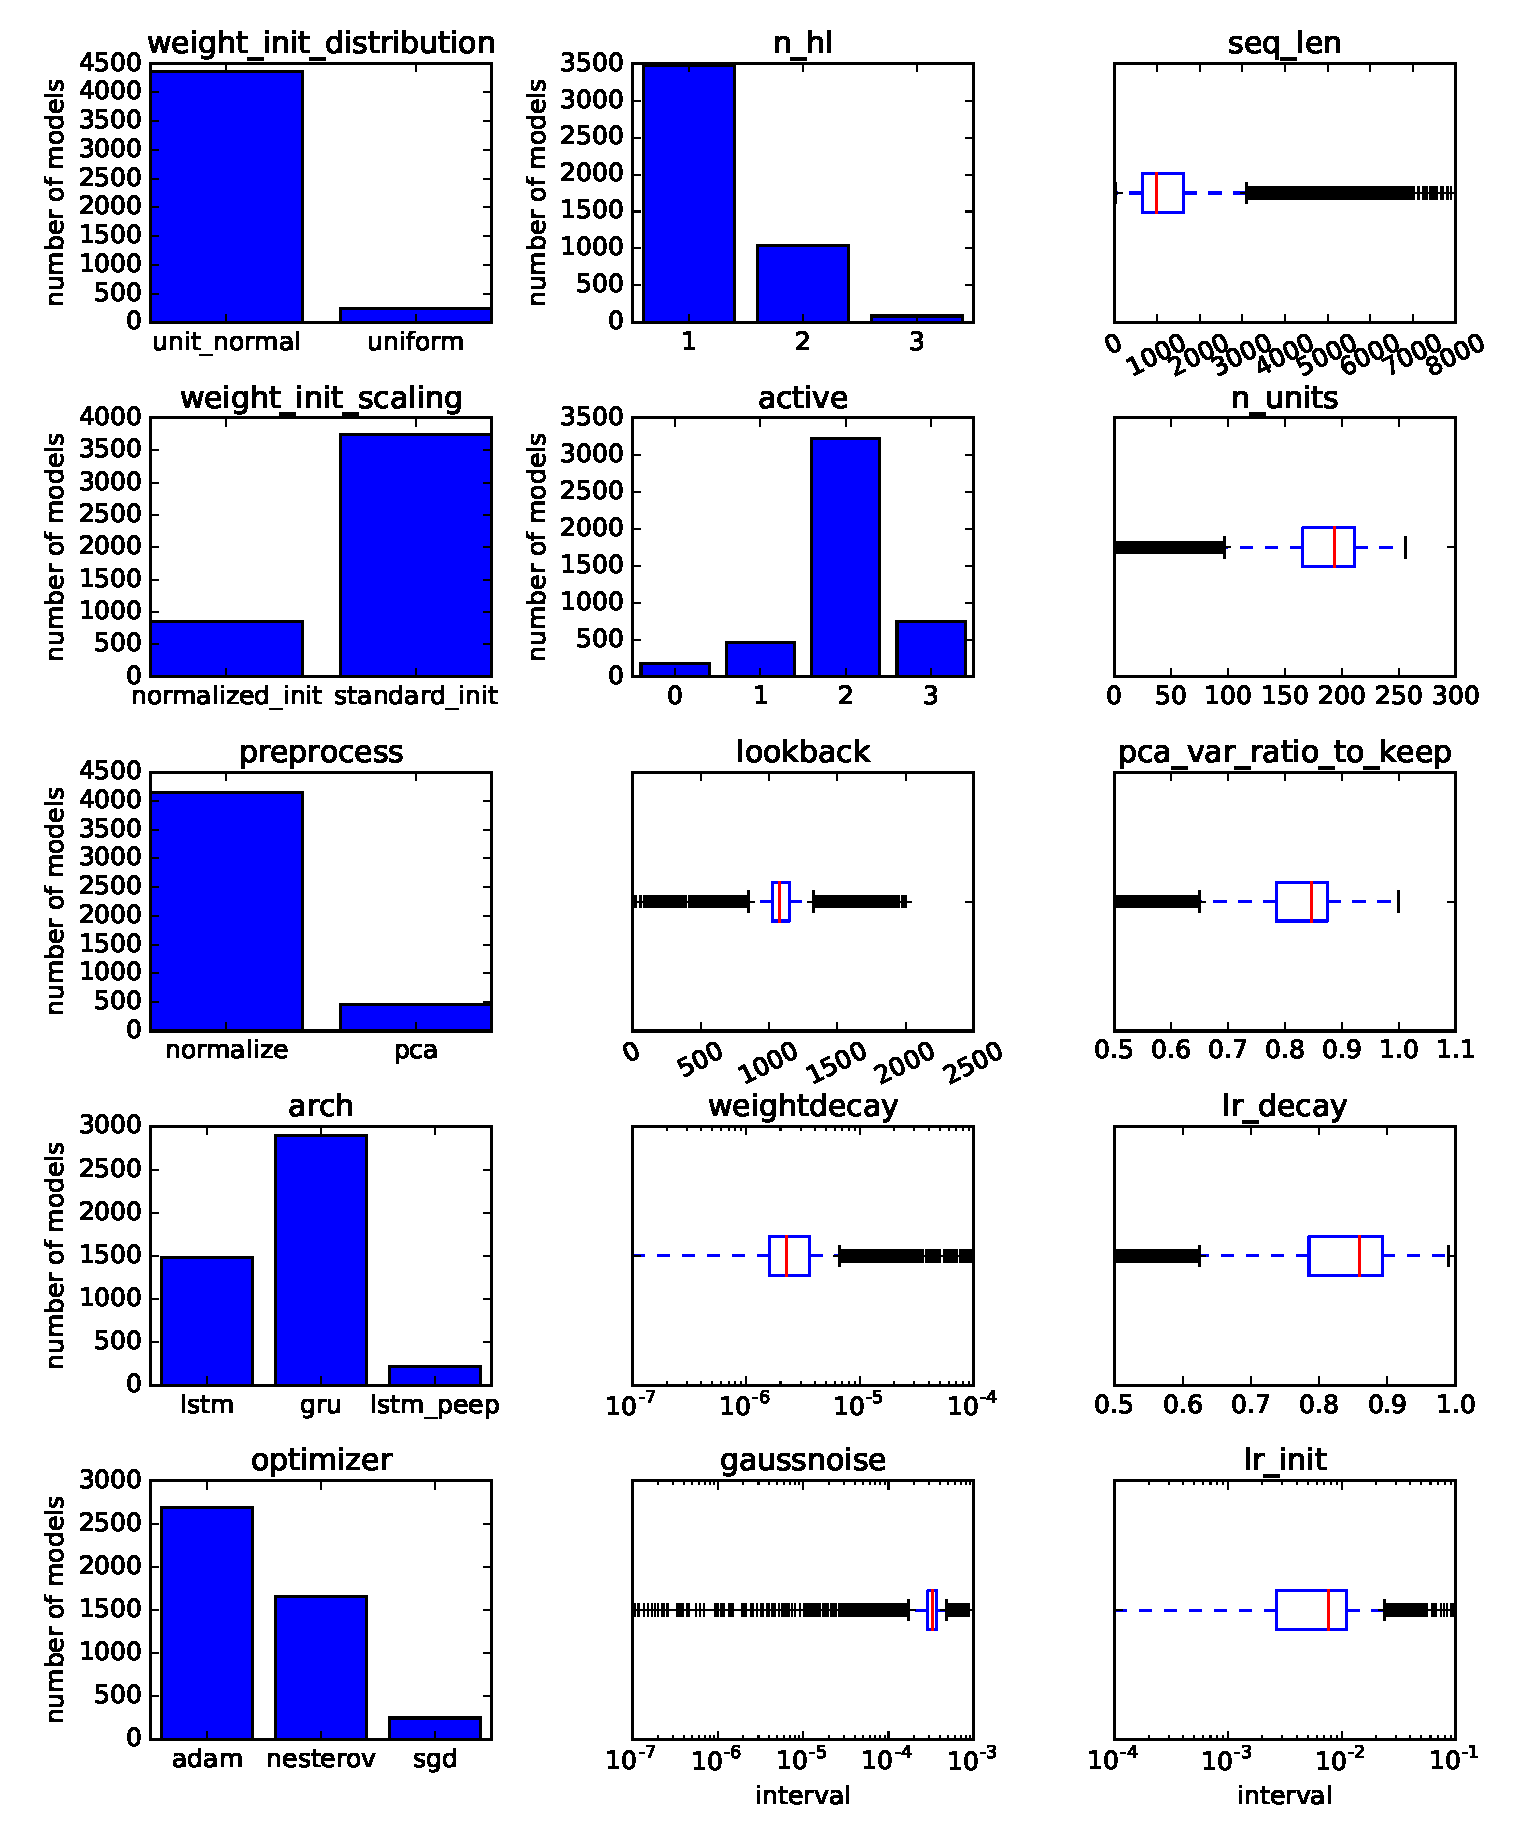
\includegraphics[width=\columnwidth]{evaluation/yoke_paramdist.eps}
	\caption{Bar plots and box plots depicting the distribution of each hyper-parameter over all \gls{pso} iterations (from experiment 4)}
	\label{fig:yoke_param_dist}
\end{figure}
\begin{figure}[!hbt]
	\centering
	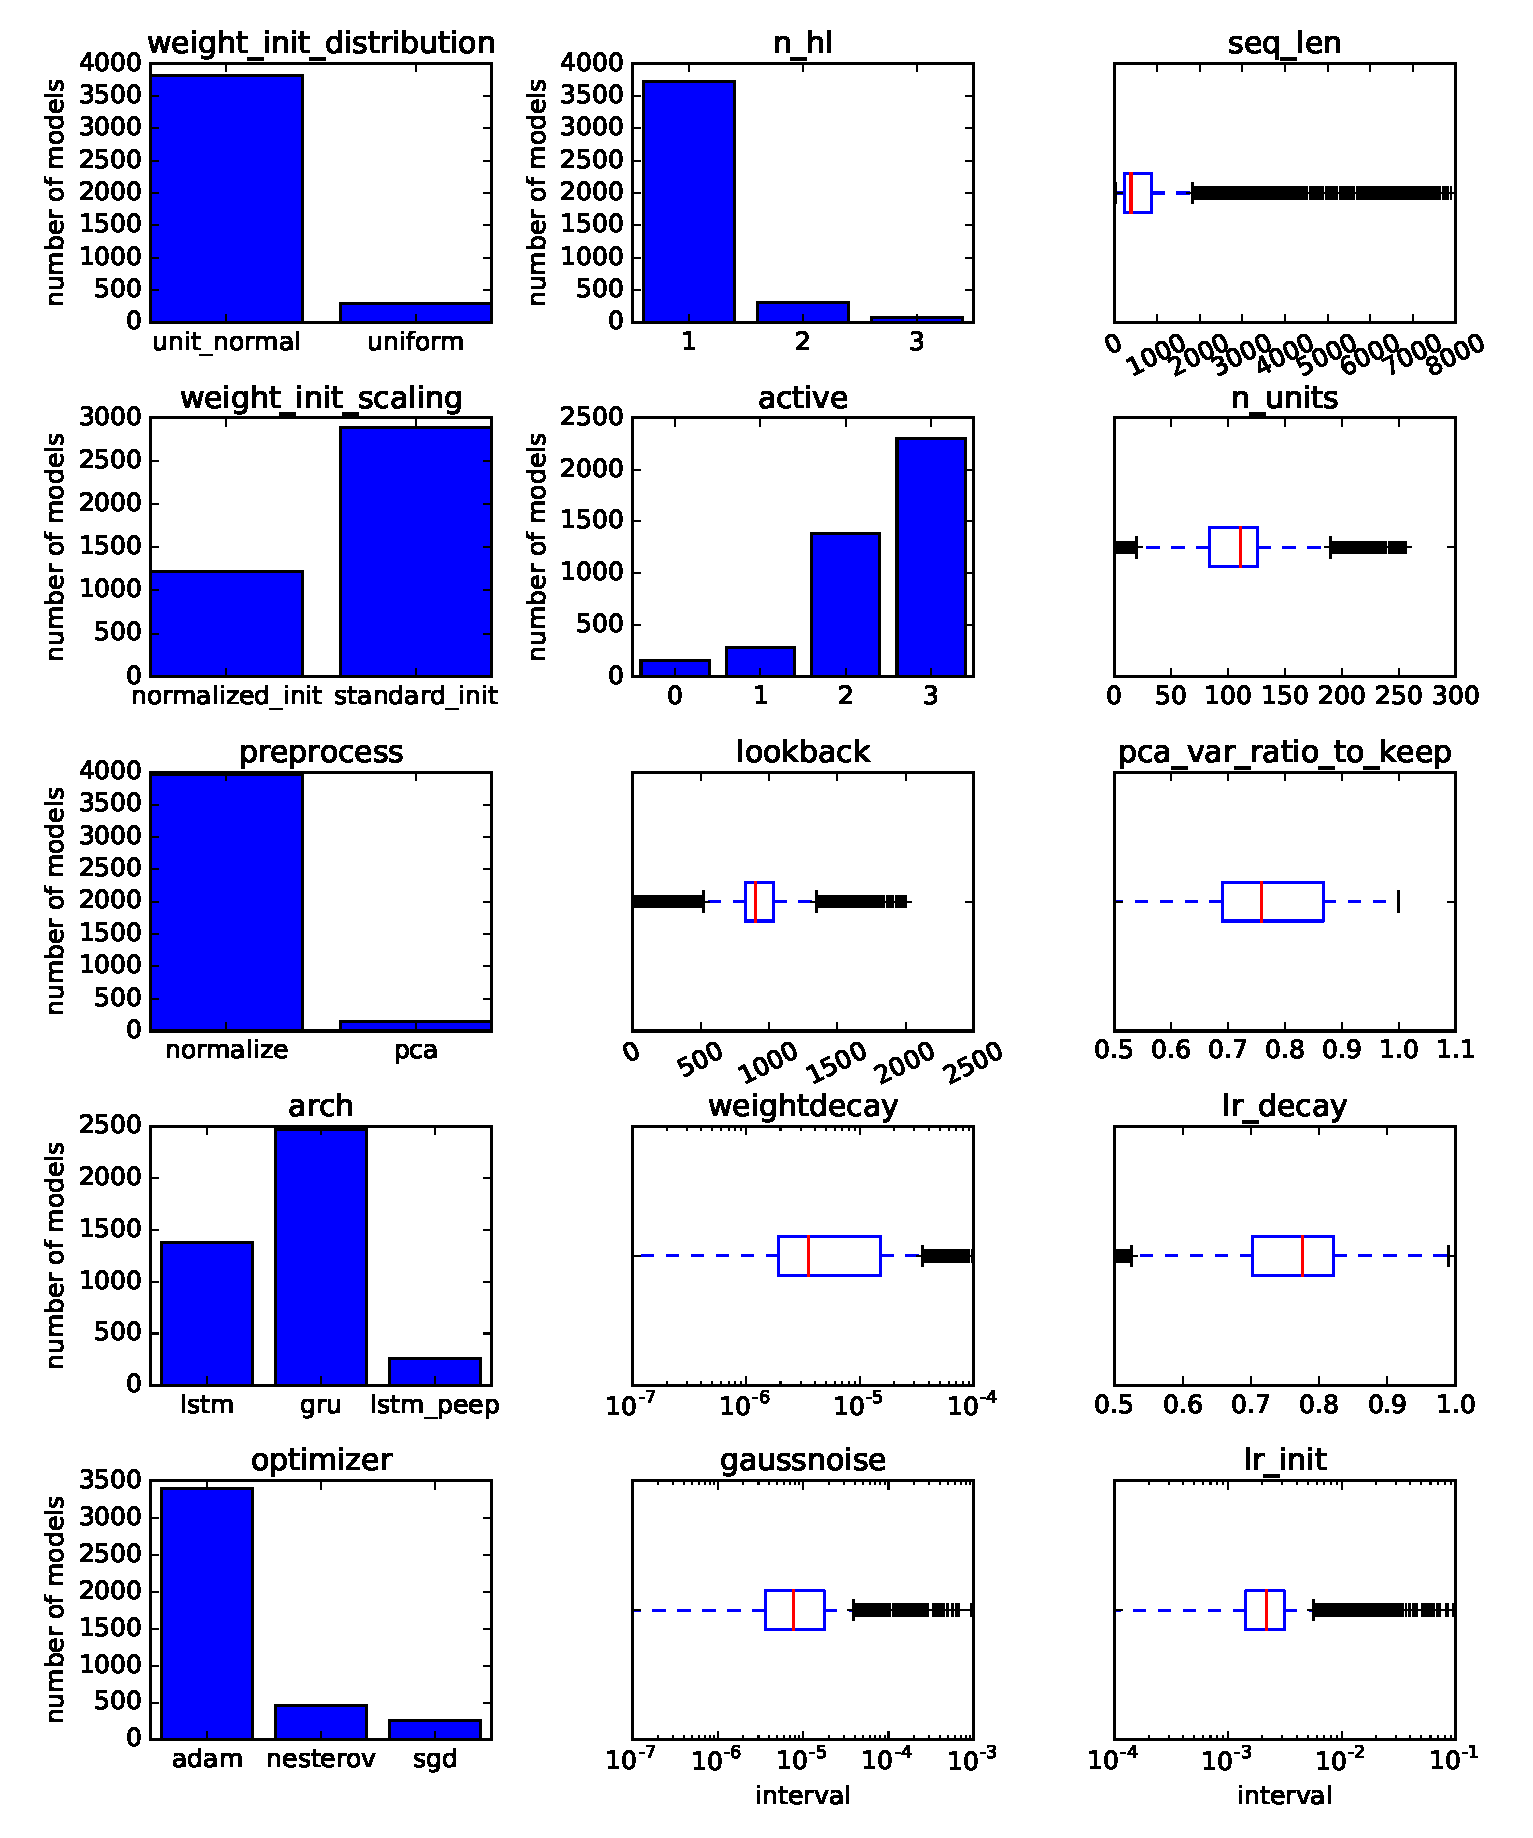
\includegraphics[width=\columnwidth]{evaluation/teeth_paramdist.eps}
	\caption{Bar plots and box plots depicting the distribution of each hyper-parameter over all \gls{pso} iterations (from experiment 5)}
	\label{fig:teeth_param_dist}
\end{figure}
\begin{figure}[!hbt]
	\centering
	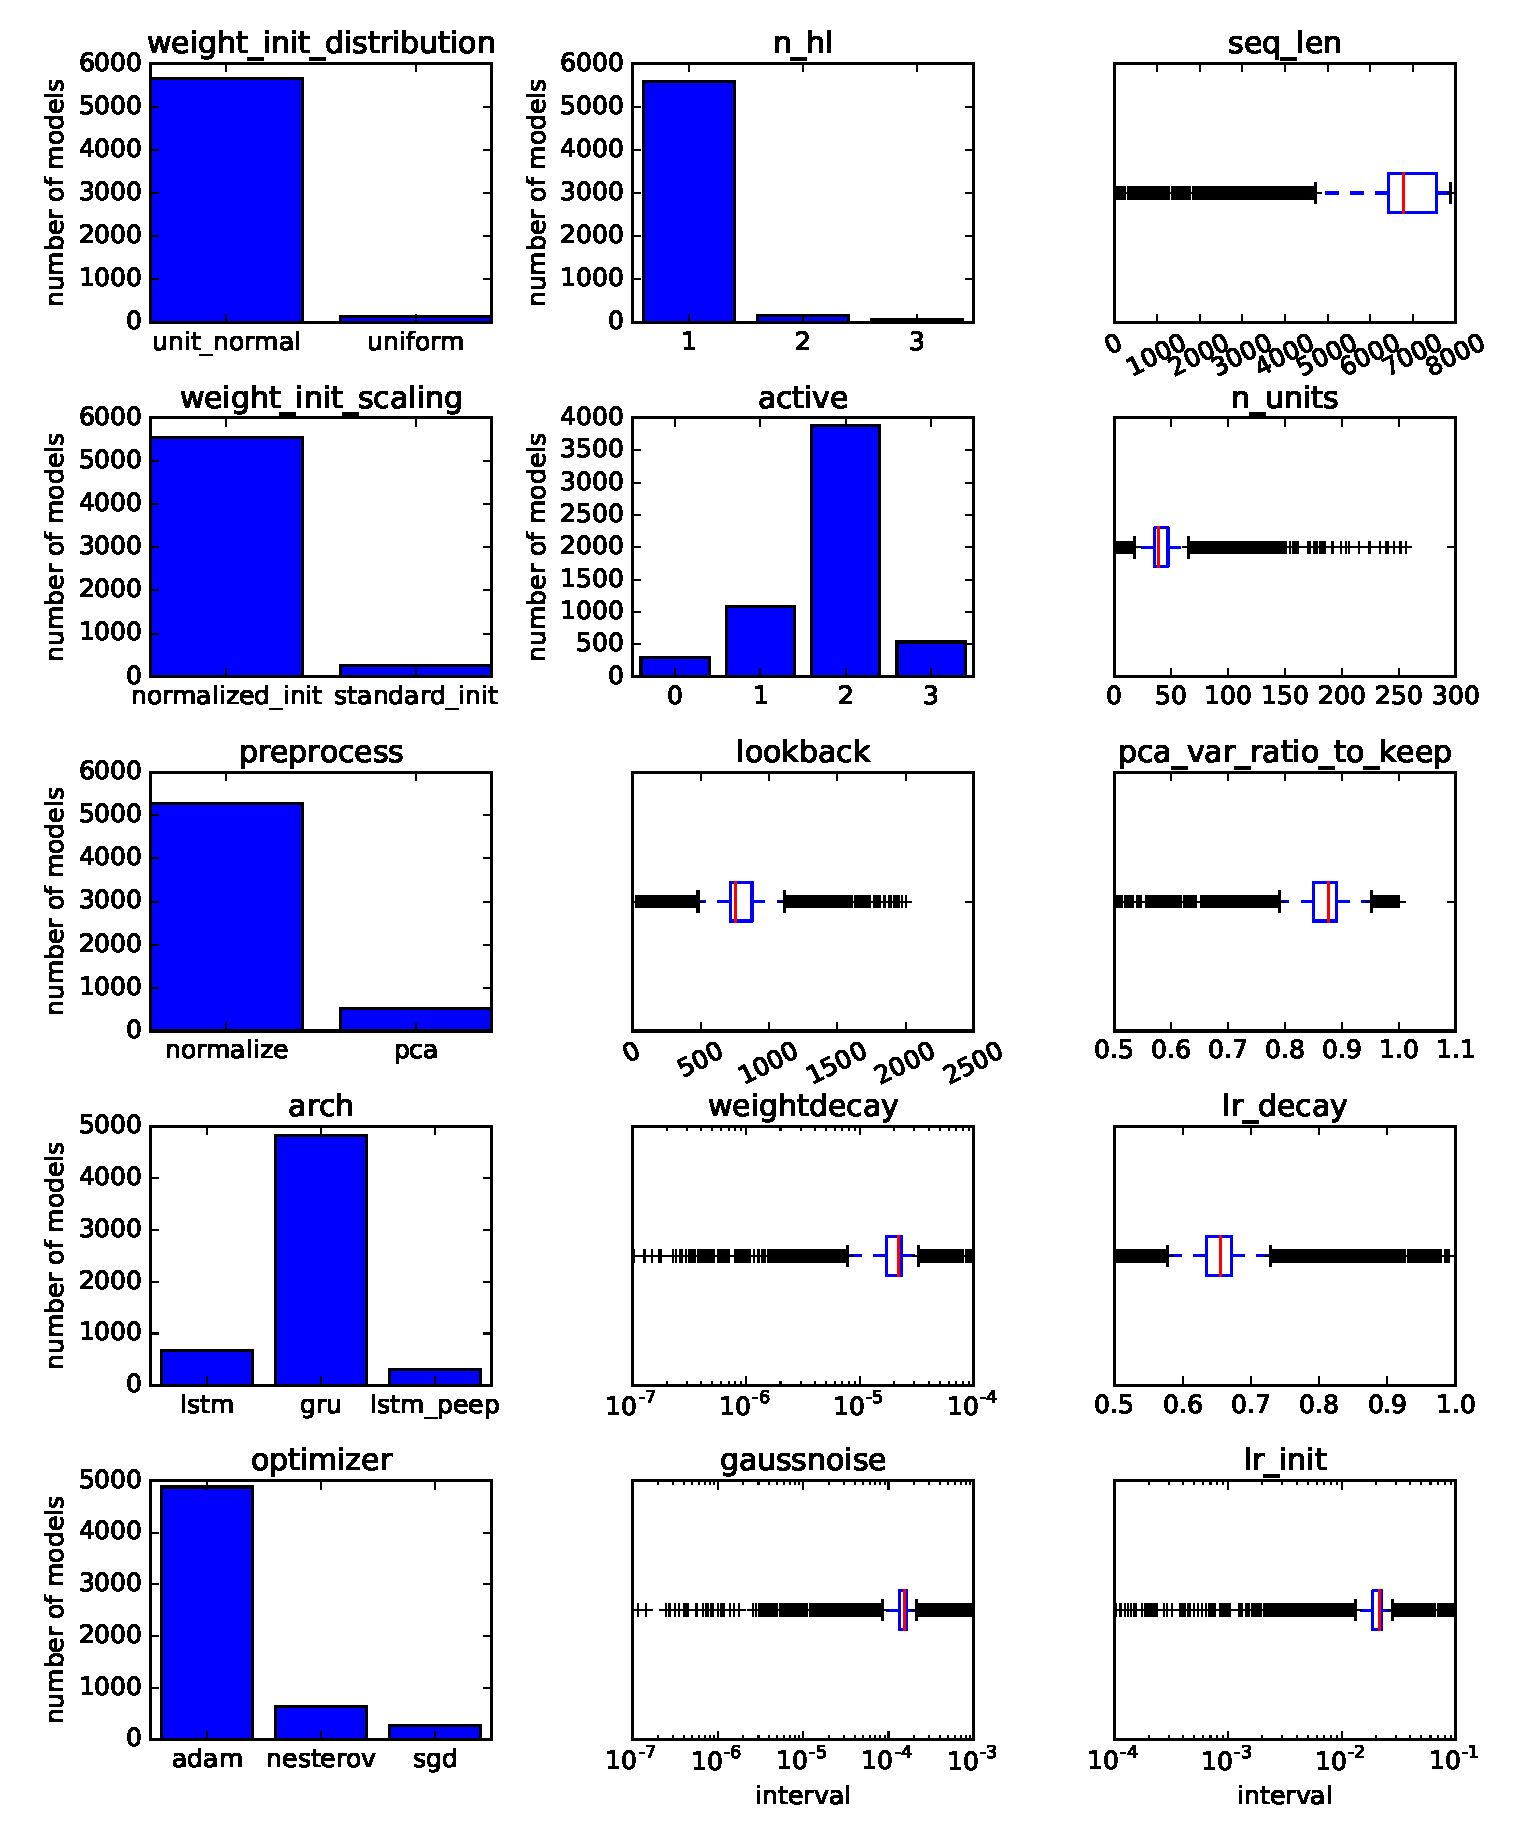
\includegraphics[width=\columnwidth]{evaluation/winding_paramdist.eps}
	\caption{Bar plots and box plots depicting the distribution of each hyper-parameter over all \gls{pso} iterations (from experiment 6)}
	\label{fig:winding_param_dist}
\end{figure}\clearpage

\section{Parameter Variance Trends}
\label{app:param_var}

Parameter variance trends encompass fig. \ref{fig:stator_var}, \ref{fig:pm_var}, \ref{fig:yoke_var}, \ref{fig:teeth_var} and \ref{fig:winding_var}.
\begin{figure}[!hbt]
	\centering
	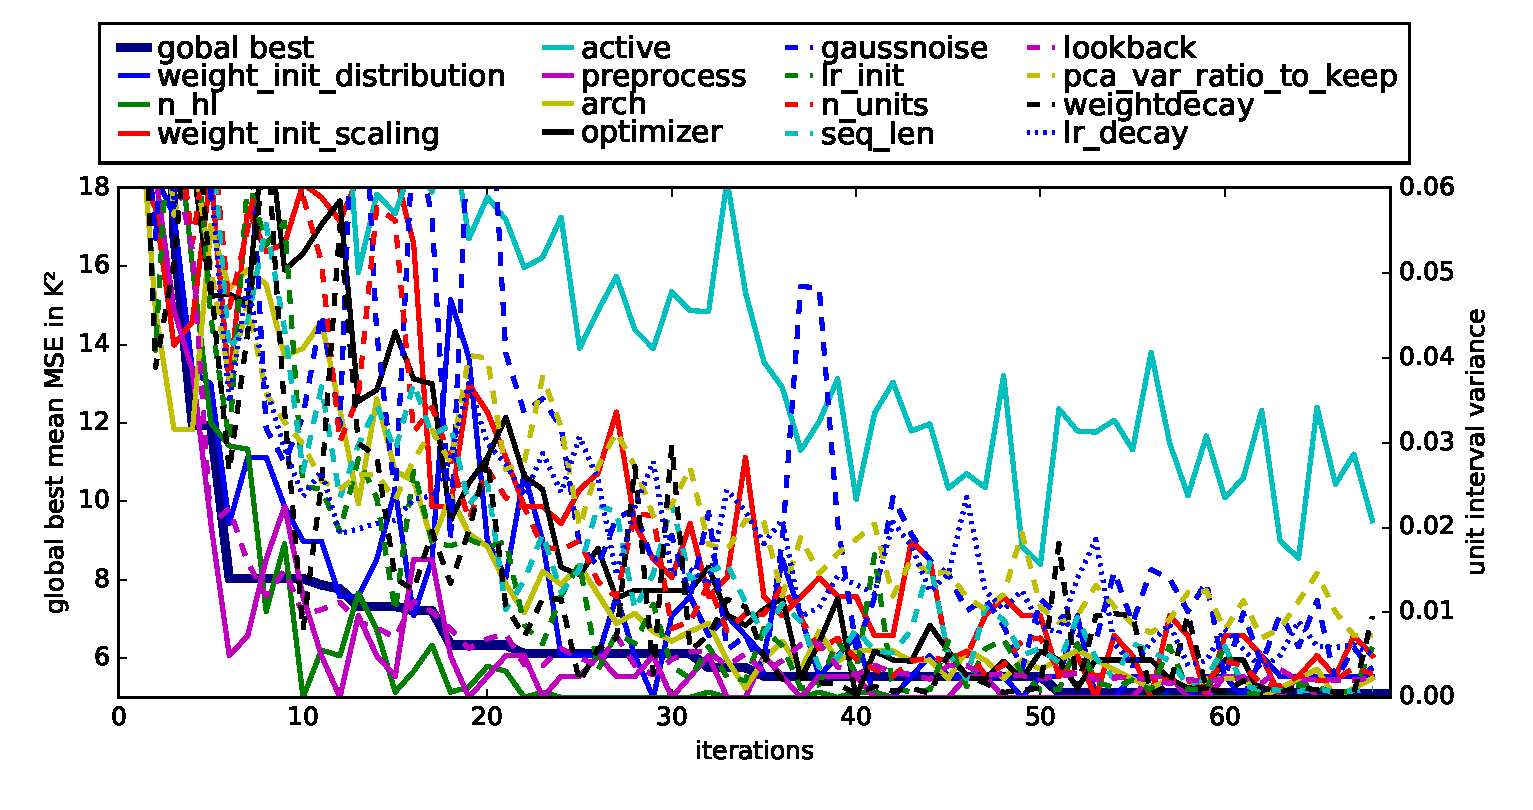
\includegraphics[width=\textwidth]{evaluation/stator_var.eps}
	\caption{Hyper-parameter variance over \gls{pso} iterations (from experiment 2)}
	\label{fig:stator_var}
\end{figure}
\begin{figure}[!hbt]
	\centering
	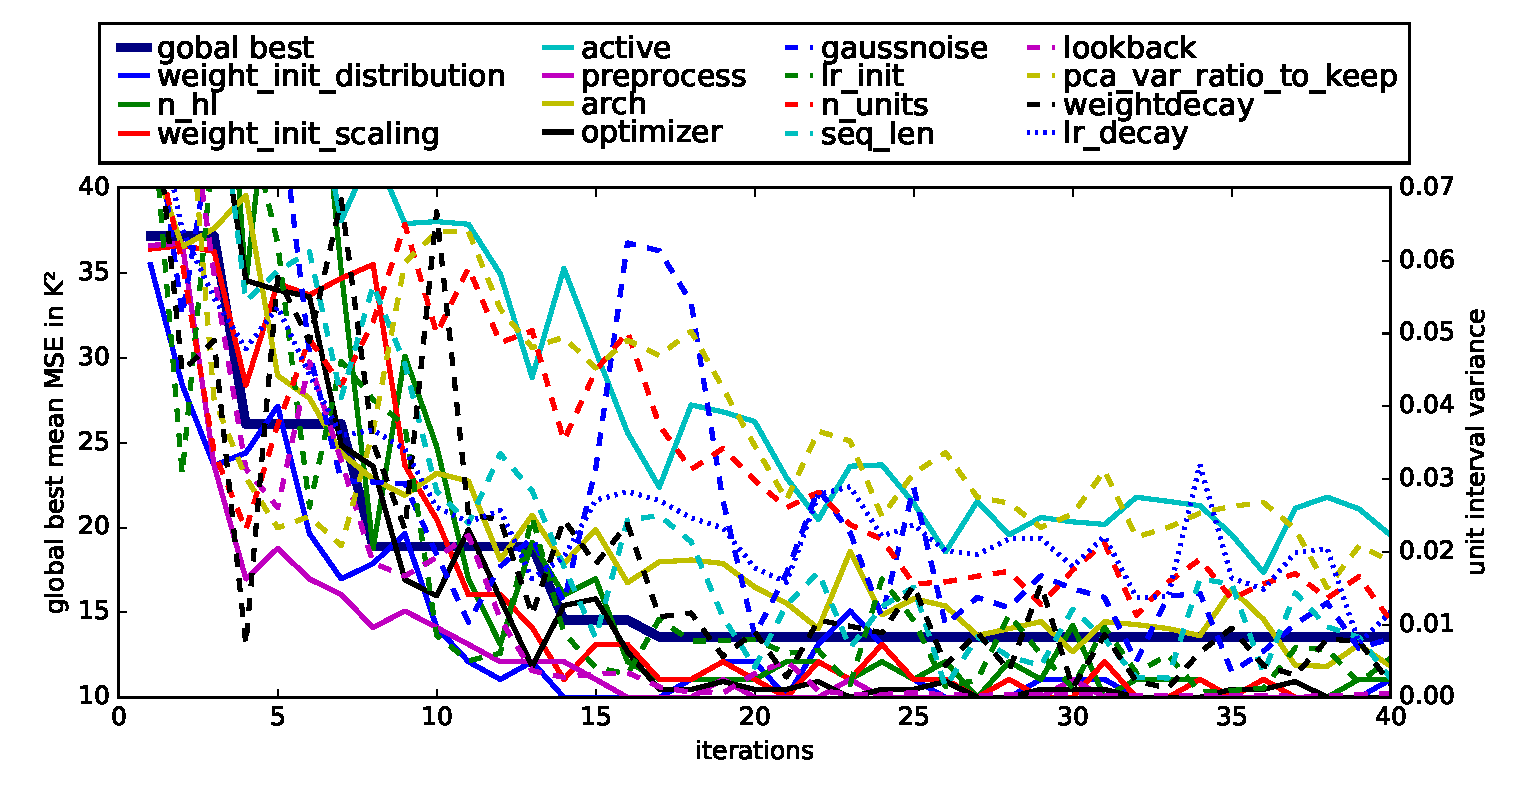
\includegraphics[width=\textwidth]{evaluation/pm_var.eps}
	\caption{Hyper-parameter variance over \gls{pso} iterations (from experiment 3)}
	\label{fig:pm_var}
\end{figure}
\begin{figure}[!hbt]
	\centering
	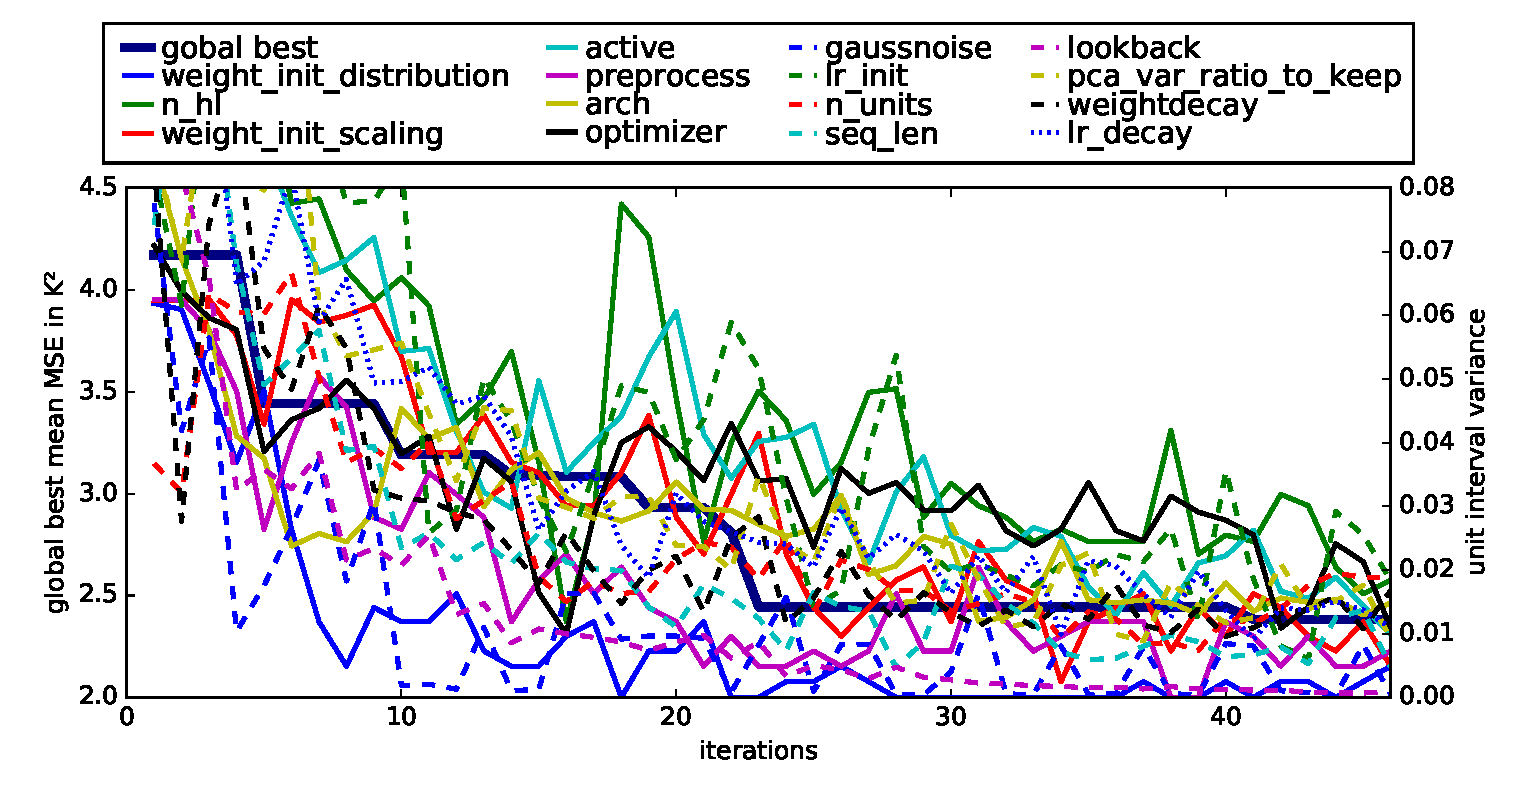
\includegraphics[width=\textwidth]{evaluation/yoke_var.eps}
	\caption{Hyper-parameter variance over \gls{pso} iterations (from experiment 4)}
	\label{fig:yoke_var}
\end{figure}
\begin{figure}[!hbt]
	\centering
	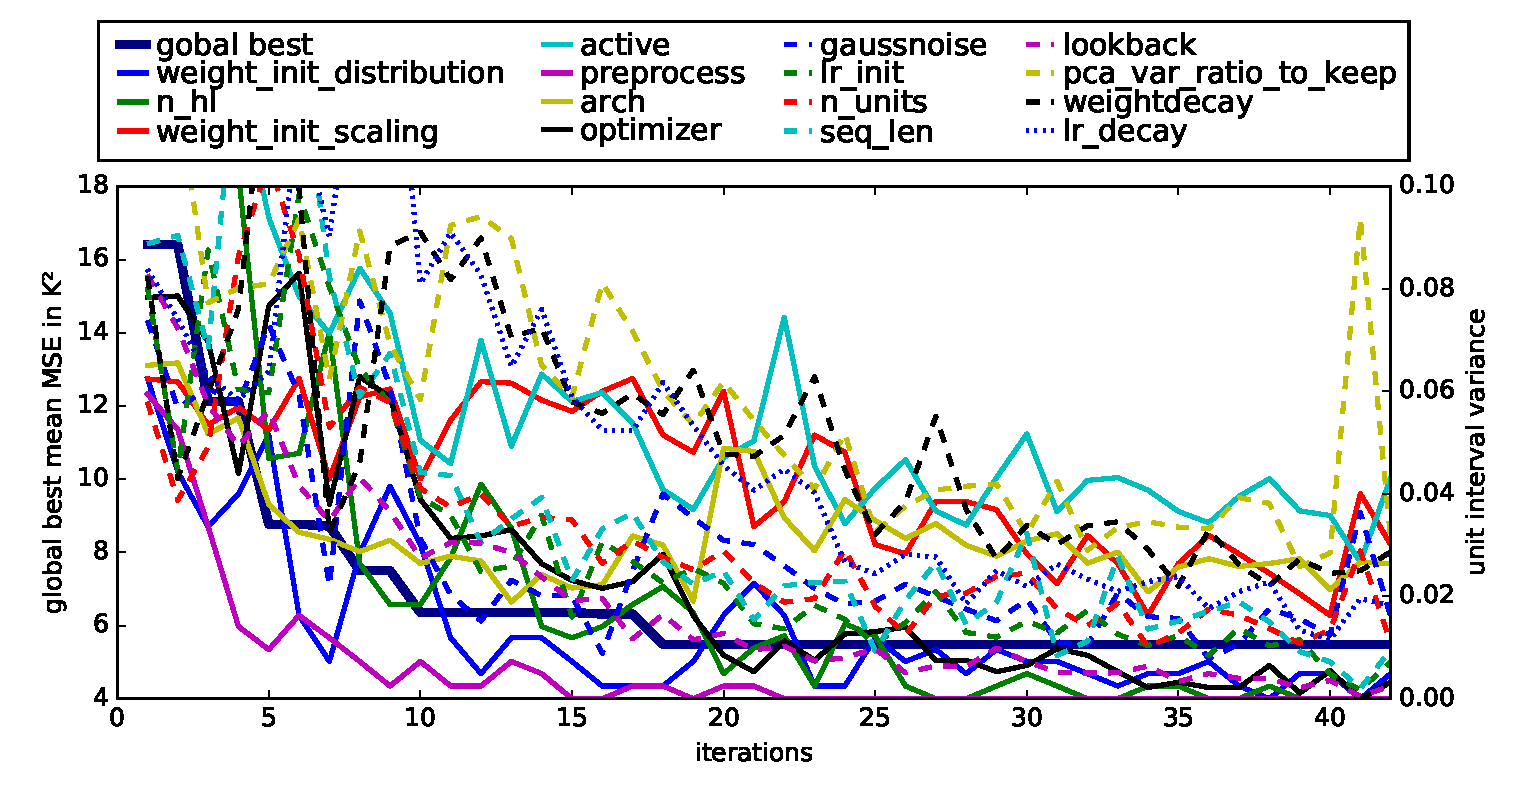
\includegraphics[width=\textwidth]{evaluation/teeth_var.eps}
	\caption{Hyper-parameter variance over \gls{pso} iterations (from experiment 5)}
	\label{fig:teeth_var}
\end{figure}
\begin{figure}[!hbt]
	\centering
	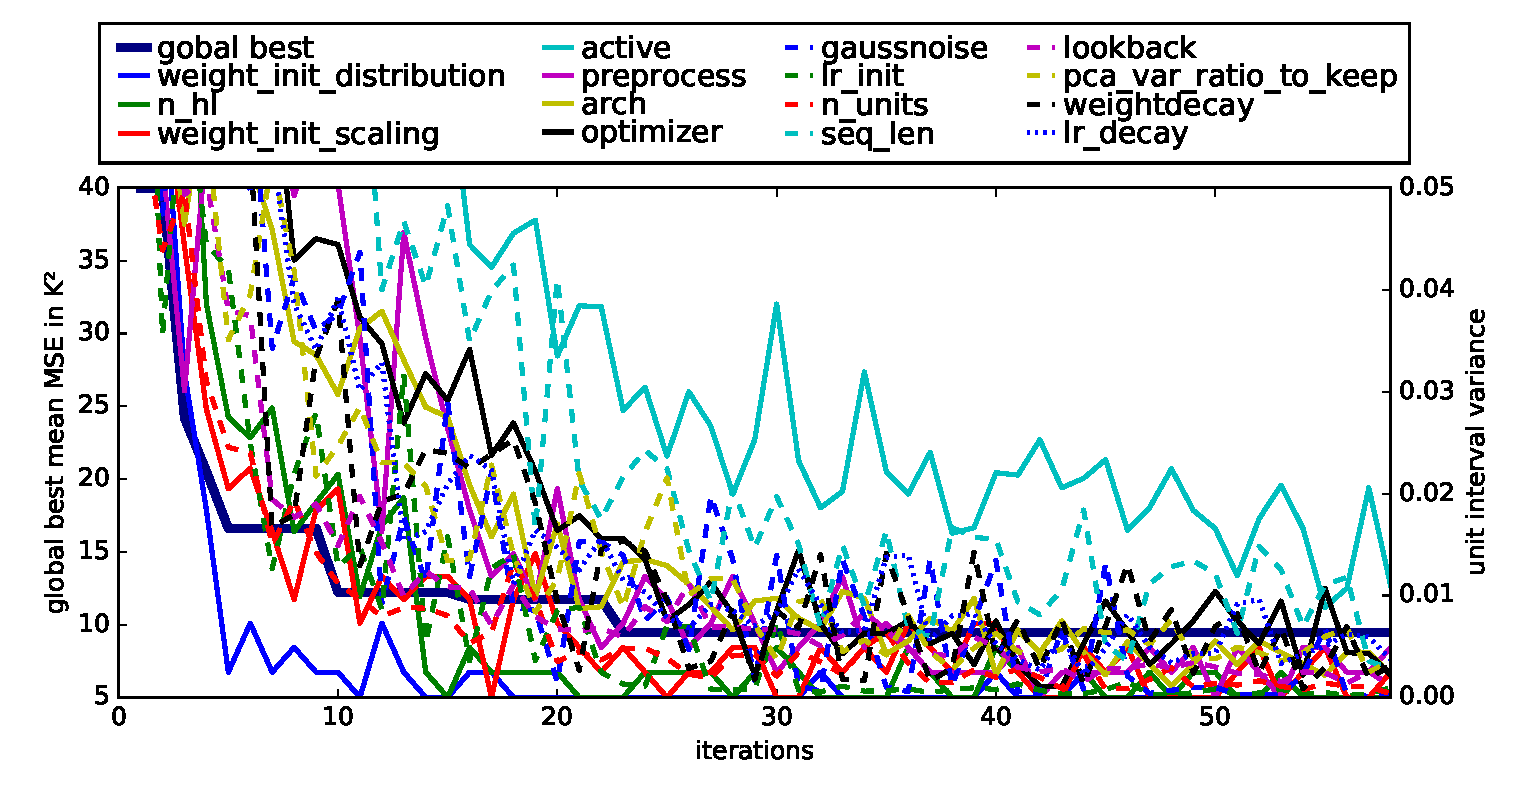
\includegraphics[width=\textwidth]{evaluation/winding_var.eps}
	\caption{Hyper-parameter variance over \gls{pso} iterations (from experiment 6)}
	\label{fig:winding_var}
\end{figure}\clearpage

\section{Sensitivity Analyses}
\label{app:sensitivity}
\begin{table}[h]
	\caption{Sensitivity analysis for experiment 1}
	\label{tab:alltargets_sensitivity}
	\centering
	\begin{tabular}{ C{2.5cm} C{2.5cm} c c}
		\toprule
		\multicolumn{2}{c}{optimum: \SI{33.16}{\kelvin\squared}}&\multicolumn{2}{c}{95\,\% confidence interval: $\pm$ 2.3\,K\textsuperscript{2}}\\
		\midrule
		 hyper-parameter & alternatives & test score estimates in K\textsuperscript{2} & $\Delta$ w.r.t. baseline in K\textsuperscript{2}\\
		 \midrule
		 arch				& \gls{gru}/ \gls{lstm}\_peepholes& 66.79/ 344.84 		& 33.63/ 311.68 \\
		 n\_hl				& 2 							& 124.41 				& 91.25 \\
		 n\_units				& 21/ 57						& 41.93/ 32.66 		& 8.77/ -0.5 \\
		 opt					& \gls{adam}/ \gls{sgd} 			& 59.66/ 40.08 		& 26.5/ 6.92 \\
		 seq\_len				& 7015/ 7880 					& 38.51/ 34.58 		& 5.35/ 1.42\\
		 lookback				& 737/ 1137 					& 40.92/ 35.16 		& 7.76/ 2.0\\
		 lr\_init				&\num{2e-4}					& 37.15				& 3.99\\
		 lr\_decay 			& 0.93/ 0.99					& 40.49/ 34.32			& 7.33/ 1.16\\
		 preprocess 			& \gls{pca}: 0.5/ 1.0				& 248.49/ 50.9			& 215.33/ 17.74\\
		 weight init. distribution& uniform					& 111.23				& 78.07\\
		 weight init. scaling 	& standard 					& 64.17 				& 31.01\\
		 active 				& 0/ 1/ 2 						& 35.41/ 35.88/ 35.02	& 2.25/ 2.72/ 1.86\\
		  \bottomrule
	\end{tabular}
\end{table}

\begin{table}[h]
	\caption{Sensitivity analysis for experiment 2}
	\label{tab:stator_sensitivity}
	\centering
	\begin{tabular}{ C{2.5cm} C{2.5cm} c c}
		\toprule
		\multicolumn{2}{c}{optimum: \SI{12.11}{\kelvin\squared}}&\multicolumn{2}{c}{95\,\% confidence interval: $\pm$ 2.53\,K\textsuperscript{2}}\\
		\midrule
		 hyper-parameter & alternatives & test score estimates in K\textsuperscript{2} & $\Delta$ w.r.t. baseline in K\textsuperscript{2}\\
		 \midrule
		 arch				& \gls{lstm}/ \gls{lstm}+peepholes& 23.5/ 375.24 		& 11.39/ 363.13 \\
		 n\_hl				& 2 							& 222.69 				& 210.58 \\
		 n\_units				& 73/ 201						& 18.25/ 142.47 		& 6.14/ 130.36 \\
		 opt					& nesterov/ \gls{sgd} 			& 42.76/ 17.83 		& 30.65/ 5.72 \\
		 seq\_len				& 6507/ 7880					& 13.74/ 24.97 		& 1.63/ 12.86\\
		 lookback				& 622/ 1022 					& 20.49/ 14.39 		& 8.38/ 2.28\\
		 lr\_init				& \num{8.62e-3}/ \num{3.43e-2}	& 13.31/ 196.85		& 1.2/ 184.74\\
		 lr\_decay 			& 0.92/ 0.99					& 17.31/ 15.22			& 5.2/ 3.11\\
		 preprocess 			& \gls{pca}: 0.5/ 1.0				& 229.96/ 47.64		& 217.85/ 35.53\\
		 weight init. distribution& uniform					& 138.3				& 126.19\\
		 weight init. scaling 	& standard 					& 16.48	 			& 4.37\\
		 active 				& 0/ 2/ 3 						& 13.51/ 14.83/ 18.72	& 1.4/ 2.72/ 6.61\\
		  \bottomrule
	\end{tabular}
\end{table}

\begin{table}[h]
	\caption{Sensitivity analysis for experiment 3}
	\label{tab:pm_sensitivity}
	\centering
	\begin{tabular}{ C{2.5cm} C{2.5cm} c c}
		\toprule
		\multicolumn{2}{c}{optimum: \SI{38.41}{\kelvin\squared}}&\multicolumn{2}{c}{95\,\% confidence interval: $\pm$ 2.98\,K\textsuperscript{2}}\\
		\midrule
		 hyper-parameter & alternatives & test score estimates in K\textsuperscript{2} & $\Delta$ w.r.t. baseline in K\textsuperscript{2}\\
		 \midrule
		 arch				& \gls{lstm}/ \gls{lstm}+peepholes& 47.19/ 183.93 		& 8.78/ 145.52 \\
		 n\_hl				& 2 							& 196.07				& 157.66 \\
		 n\_units				& 86/ 236						& 44.51/ 180.37		& 6.1/ 141.96 \\
		 opt					& nesterov/ \gls{sgd} 			& 85.57/ 66.97			& 47.16/ 28.56  \\
		 seq\_len				& 7095 						& 30.02		 		& -8.21\\
		 lookback				& 1800 						& 40.47		 		& 2.06\\
		 lr\_init				&\num{6.28e-3}/ \num{2.5e-2}	& 78.79/ 219.45		& 40.38/ 181.04\\
		 lr\_decay 			& 0.9/ 0.99					& 41.4/42.88			& 2.99/ 4.47\\
		 preprocess 			& \gls{pca}: 0.5/ 1.0				& 115.6/ 68.96			& 77.19/ 30.55\\
		 weight init. distribution& uniform					& 295.97				& 257.56\\
		 weight init. scaling 	& standard 					& 73.79				& 35.38\\
		 active 				& 0/ 2/ 3						& 39.67/ 38.87/ 38.14	& 1.26/ 0.46/ -0.27\\
		  \bottomrule
	\end{tabular}
\end{table}

\begin{table}[h]
	\caption{Sensitivity analysis for experiment 4}
	\label{tab:yoke_sensitivity}
	\centering
	\begin{tabular}{ C{2.5cm} C{2.5cm} c c}
		\toprule
		\multicolumn{2}{c}{optimum: \SI{7.8}{\kelvin\squared}}&\multicolumn{2}{c}{95\,\% confidence interval: $\pm$ 2.15\,K\textsuperscript{2}}\\
		\midrule
		 hyper-parameter & alternatives & test score estimates in K\textsuperscript{2} & $\Delta$ w.r.t. baseline in K\textsuperscript{2}\\
		 \midrule
		 arch				& \gls{lstm}/ \gls{lstm}+peepholes& 28.17/ 265.32 		& 20.37/ 257.52 \\
		 n\_hl				& 2 							& 98.57 				& 90.77 \\
		 n\_units				& 142/ 300					& 6.86/ 17.64 			& -0.94/ 9.84 \\
		 opt					& nesterov/ \gls{sgd} 			& 14.79/ 8.95 			& 6.99/ 1.15  \\
		 seq\_len				& 77/ 1647 					& 12.38/ 29.35 		& 4.58/ 21.55\\
		 lookback				& 860/ 1260 					& 7.36/ 6.3	 		& -0.44/ -1.5\\
		 lr\_init				&\num{5.65e-3}/ \num{2.25e-2}	& 6.78/ 103.95			& -1.02/ 96.15\\
		 lr\_decay 			& 0.85/ 0.95					& 6.17/ 5.75			& -1.63/ -2.05\\
		 preprocess 			& \gls{pca}: 0.5/ 1.0				& 353.53/ 81.3			& 345.73/ 73.5\\
		 weight init. distribution& uniform					& inf.				& inf.\\
		 weight init. scaling 	& normalized 					& 49.18 				& 41.38\\
		 active 				& 0/ 1/ 3						& 5.64/ 15.10/ 7.84		& -2.16/ 7.3/ 0.04\\
		  \bottomrule
	\end{tabular}
\end{table}

\begin{table}[h]
	\caption{Sensitivity analysis for experiment 5}
	\label{tab:teeth_sensitivity}
	\centering
	\begin{tabular}{ C{2.5cm} C{2.5cm} c c}
		\toprule
		\multicolumn{2}{c}{optimum: \SI{12.41}{\kelvin\squared}}&\multicolumn{2}{c}{95\,\% confidence interval: $\pm$ 2.22\,K\textsuperscript{2}}\\
		\midrule
		 hyper-parameter & alternatives & test score estimates in K\textsuperscript{2} & $\Delta$ w.r.t. baseline in K\textsuperscript{2}\\
		 \midrule
		 arch				& \gls{lstm}/ \gls{lstm}+peepholes& 24.63/ 260.72		&  12.22/ 248.31\\
		 n\_hl				& 2 							& 18.23				& 5.82 \\
		 n\_units				& 69/ 189						& 14.88/ 12.66			& 2.47/ 0.25 \\
		 opt					& nesterov/ \gls{sgd} 			& 17.15/ 19.3 			& 4.74/ 6.89  \\
		 seq\_len				& 30/ 1145 					& 18.84/ 20.01 		& 6.43/ 7.6\\
		 lookback				& 680/ 1080 					& 19.35/ 14.24 		& 6.94/ 1.83\\
		 lr\_init				&\num{1.1e-3}/ \num{4.39e-3}	& 15.91/ 17.68			& 3.5/ 5.27\\
		 lr\_decay 			& 0.74/ 0.84					& 17.73/ 16.42			& 5.32/ 4.01\\
		 preprocess 			& \gls{pca}: 0.5/ 1.0				& 340.34/ 189.23		& 327.93/ 176.82\\
		 weight init. distribution& uniform					& inf.				& inf.\\
		 weight init. scaling 	& normalized 					& 21.92				& 9.51\\
		 active 				& 0/ 1/ 3						& 20.89/ 16.0/ 14.12	& 8.48/ 3.59/ 1.71\\
		  \bottomrule
	\end{tabular}
\end{table}

\begin{table}[h]
	\caption{Sensitivity analysis for experiment 6}
	\label{tab:winding_sensitivity}
	\centering
	\begin{tabular}{ C{2.5cm} C{2.5cm} c c}
		\toprule
		\multicolumn{2}{c}{optimum: \SI{21.53}{\kelvin\squared}}&\multicolumn{2}{c}{95\,\% confidence interval: $\pm$ 2.82\,K\textsuperscript{2}}\\
		\midrule
		 hyper-parameter & alternatives & test score estimates in K\textsuperscript{2} & $\Delta$ w.r.t. baseline in K\textsuperscript{2}\\
		 \midrule
		 arch				& \gls{lstm}/ \gls{lstm}+peepholes& 61.96/ 469.27		& 40.43/ 447.74\\
		 n\_hl				& 2 							& 38.37				& 16.84 \\
		 n\_units				& 23/ 62						& 29.05/ 18.85			& 7.85/ -2.68\\
		 opt					& nesterov/ \gls{sgd} 			& 41.41/ 41.13			& 6.94/ 19.6\\
		 seq\_len				& 5885/ 7455 					& 28.47/ 26.24 		& 6.94/ 4.71\\
		 lookback				& 532/932 					& 28.27/ 22.94 		& 6.74/ 1.41\\
		 lr\_init				&\num{1.09e-2}/ \num{4.33e-2}	& 25.64/ 44.89			& 4.11/ 23.36\\
		 lr\_decay 			& 0.61/ 0.7					& 23.0/ 20.86			& 1.47/ -0.67\\
		 preprocess 			& \gls{pca}: 0.5/ 1.0				& 262.79/ 589.68		& 241.26/ 568.15\\
		 weight init. distribution& uniform					& 115.64				& 94.11\\
		 weight init. scaling 	& standard 					& 46.45				& 24.92\\
		 active 				& 0/ 1/ 3						& 24.16/ 20.30/ 21.01	& 2.63/ -1.23/ -0.52\\
		  \bottomrule
	\end{tabular}
\end{table}

